\documentclass[10pt, oneside]{scrartcl}   	% use "amsart" instead of "article" for AMSLaTeX format
\usepackage[top=2cm,right=2cm,bottom=2.5cm,left=2cm]{geometry}                		% See geometry.pdf to learn the layout options. There are lots.
% \usepackage[top=4cm,right=4cm,bottom=4cm,left=4cm]{geometry}
\geometry{letterpaper}                   		% ... or a4paper or a5paper or ... 
%\geometry{landscape}                		% Activate for for rotated page geometry
%\usepackage[parfill]{parskip}    		% Activate to begin paragraphs with an empty line rather than an indent
\usepackage[parfill]{parskip}
\usepackage{graphicx}				% Use pdf, png, jpg, or eps� with pdflatex; use eps in DVI mode
\usepackage{subfig}
								% TeX will automatically convert eps --> pdf in pdflatex
\usepackage{amssymb}
\usepackage{amsmath}
\usepackage{natbib}

\usepackage[TS1,T1]{fontenc}
%\usepackage{fourier, heuristica}
\usepackage{array, booktabs}
\usepackage[x11names]{xcolor}
\usepackage{colortbl}
\usepackage{caption}
\usepackage{bbm}
\usepackage{amssymb}
\usepackage{amsmath}
\usepackage{mathtools}
\usepackage{float}
\DeclareCaptionFont{blue}{\color{LightSteelBlue3}}

\newcommand{\foo}{\color{LightSteelBlue3}\makebox[0pt]{\textbullet}\hskip-0.5pt\vrule width 1pt\hspace{\labelsep}}

\definecolor{light-gray}{gray}{0.7}

\title{Automatic Metadata Extraction: The High Energy Physics Use Case}
\author{Joseph Boyd}
% \date{}							% Activate to display a given date or no date

\renewcommand{\thesubfigure}{\thefigure.\arabic{subfigure}}

\begin{document}

\maketitle

\tableofcontents

\section{Introduction} % 3 - 10

\subsection{Motivation}
\subsection{Aims}
\subsection{Main Results}
\subsection{Outline}
\section{Supervised Sequence Learning}
\emph{In this section we present the state-of-the-art technique for metadata extraction, conditional random fields (CRF). For completeness, we include a background history of related machine learning techniques and their optimisation algorithms. Notably, we pinpoint the piece of the mathematical model relevant to our work on feature engineering. Finally, we describe Wapiti, a general-purpose ``engine'' for training and applying CRF models.}

\begin{enumerate}
\item HMMs
\item logistic regressions, (and optimisation thereof)
\item Maxent and how they differ to CRFs ~\cite{peng2006information}
\item Inference algorithms
\item l-bfgs
\item mention sequence learning, graphical models, random fields, Hammersley-Clifford
\item define discriminative etc.
\item feature engineering
\item segue into Wapiti
\end{enumerate}

\subsection{Log-linear Models}
\subsection{Graphical Models}
\subsubsection{Hidden Markov Models}
\subsection{Conditional Random Fields}
\subsubsection{Feature Engineering}
\subsubsection{Wapiti}
Lack of support for numeric features imposes constraints our feature engineering. Any numeric-based idea must be discretised\footnote{this is a footnote, and it's crazy easy to make in latex.}.

Both approaches yield the same input data for the CRF engine, and so evaluation is in fact equivalent to prediction, despite the initial difference in input formats. Figure \ref{fig:traininput} shows an excerpt from an input file to the CRF engine for training. These features are for inputs ``January 1994'' and ``July 1996'', for training the Date model. The features range from token identity, to a variety of prefixes and punctuation features. It should be noted that OCR information is only used in higher level models, that is, the Header and Segmentation models. The input for lower-level models such as Date is plaintext, and so features are typically simple, but dictionary-based features, where information about a token is referenced in a dictionary resource within Grobid, are also used. Note the features shown are only those pertaining to the token itself. The full range of features (including those involving concatenations of the token's neighbours etc.) are defined by a set of feature templates. The feature templates for each model are contained in a separate file. An excerpt of this is shown in Figure \ref{fig:template}. These are given as a separate input to the CRF engine, and it is with these that the engine constructs all feature functions for the model. It is therefore vital that the feature extraction, which is generated by Grobid, is aligned with the template file, which is manually configured by the developer. As depicted in Figure \ref{fig:flow}, there is a strong coupling between these two parts of Grobid. The excerpt shown is from the Wapiti model, but the notation is the same for CRF++, which first standardised the syntax. This subset of five feature templates capture information about the capitalisation of a token and its neighbours. The notation has the structure, [identifier]:[\%x][row, col], where row is the offset from the current token, and col indicates the feature index. Thus, ``U50:\%[0,11]'', denotes that the feature template identified as ``U50'' takes the 11th feature for the current token (0 offset). This feature will be equal to 1 if a token is capitalised, and 0 otherwise. ``U52:\%[-1,11]'' indicates the same thing, but based on the capitalisation of the \emph{previous} token. ``U54:\%x[-1,11]/\%x[0,11]'' is a binary function for detecting the capitalisation of the current \emph{and} the following token.

Now we may see an alignment with the mathematical model. Recall a linear chain CRF is expressed in the simplest case as,

\begin{equation}
p(\textbf{y}|\textbf{x}) = \frac{p(\textbf{x}, \textbf{y})}{\sum_{y'}{p(\textbf{x}, \textbf{y}')}},
\end{equation}

where, 

\begin{equation}
p(\textbf{x}, \textbf{y}) = \text{exp} \Bigg\{\sum_t{
\sum_{i, j \in S}{
\lambda_{ij}\mathbbm{1}_{\{y_t = i\}}\mathbbm{1}_{\{y_{t-1} = j\}}
}
+ \sum_t\sum_{i \in S}\sum_{o \in O}{
\mu_{io}\mathbbm{1}_{\{y_t = i\}}\mathbbm{1}_{\{x_t = o\}}
}
}\Bigg\},
\label{eq:joint}
\end{equation}

Here $\textbf{x}$ is a sequence of observations and $\textbf{y}$ is a sequence of labels. $S$ is the set of all labels, $O$ is set of observations (the vocabulary of the tokens to be labelled). When the coefficients $\lambda_{ij} = \log p(y_t=i, y_{t - 1}=j)$ and $\mu_{ij} = \log p(y_t=i,x_t=o)$, this joint distribution is equivalent to a Hidden Markov Model (HMM), with coefficients, $\lambda_{ij}$ as transition probabilities and $\mu_{ij}$ emission probabilities. In this simple case, features are based solely on the token's identity, i.e. feature functions are an indicator function. For clarity, we may write,

\begin{equation}
p(\textbf{x}, \textbf{y}) = \text{exp} \Bigg\{
\sum_{i \in S}
\sum_{j \in S}
\lambda_{ij}
F_{ij}(\textbf{y})
+ 
\sum_{i \in S}
\sum_{o \in O}
\mu_{io}
F_{io}(\textbf{x}, \textbf{y})
\Bigg\},
\label{eq:joint}
\end{equation}

where $F_{ij} = \sum_t\mathbbm{1}_{\{y_t = i\}}\mathbbm{1}_{\{y_{t-1} = j\}}$ and $F_{io} = \sum_t\mathbbm{1}_{\{y_t = i\}}\mathbbm{1}_{\{x_t = o\}}$. In a CRF, however, we may replace the indicator function for observations with any sort of function, typically binary, extracting rich features from a token. Thus, $F_{io} = \sum_t\mathbbm{1}_{\{y_t = i\}}f_{io}(\textbf{x})$. The set of functions, $\{f_{io}\}$, are the functions that we define in the feature template files. Note that, unlike an HMM, the vocabulary is not pre-defined, it is ``discovered'' through training on samples. Therefore, the number of actual features depends on the training set itself, whereas the feature template is fixed. Since we use indicator functions, which produce a feature for every observation, we may end up with an enormous number of features. Take the Date model for example: 5815 features are produced for a single block (not counting the one representing the label), and there are seven labels. As per our formulation in (\ref{eq:joint}) we therefore have 7 * 7 ``transition'' features and 5815 * 7 ``emission'' features, totalling 40754 features. This is corroborated by the model output in Figure \ref{fig:output}. Wapiti automatically constructs this vast feature space from the inputs we provide. In the Date model, the labels are I-<day>, I-<month>, I-<year>, I-<other>, <day>, <month>, and <other>. The I (probably) stands for ``initial'', as in training these are assigned to the first tokens of this class found in the string.

\begin{figure}
\begin{verbatim}
* Initialize the model
* Summary
    nb train:    493
    nb labels:   7
    nb blocks:   5816
    nb features: 40754
* Train the model with l-bfgs
  [   1] obj=1688,58    act=16482    err=25,80\%/50,91\% time=0,08s/0,08s
  [   2] obj=1221,30    act=15580    err=19,11\%/35,50\% time=0,05s/0,12s
  [   3] obj=922,15     act=13869    err=17,20\%/33,67\% time=0,04s/0,17s
  [   4] obj=638,04     act=10845    err= 6,53\%/15,21\% time=0,04s/0,20s
  [   5] obj=478,72     act=10582    err= 5,68\%/13,59\% time=0,04s/0,24s
  [   6] obj=416,15     act=9926     err= 3,77\%/ 9,53\% time=0,04s/0,28s
\end{verbatim}
\caption{Output from training date model}
\label{fig:output}
\end{figure}

A model is typically a large file (as much as 100Mb). At the top of the file, the feature templates are declared, just as they are in the input. Because of this, that file is not required at prediction time. Following this the labels are declared. Then come two longer sections: first, the feature functions themselves as defined. Figure \ref{fig:model} shows the first 12 features produced from the first token in the first sample in the training set--``November''. Because this is the first token in the string, we see the first three feature macros, which relate to the identity of the token's predecessors, remain unresolved. The fourth, however, shows the indicator for the token. This function will be true if a token is equal to ``November''. The fifth function is an indicator for if the token's successor is equal to ``19'', and so on. The final (and usually largest) section of the model file defines the non-zero weights for the feature functions. The weights are represented in scientific notation and in hexadecimal representation, presumably to avoid arithmetic underflow (a common problem when dealing with with the computation of HMMs and related models).

\section{Automatic Metadata Extraction}
\subsection{Metadata Extraction}
\subsection{Related Work}
\subsection{GROBID}

\begin{table}[h]
\begin{tabular}{ccccc}
\hline
label		&accuracy	&precision	&recall		&f1 \\
\hline
<label>		&99.96		&100		&99.2		&99.6\\
<reference>		&99.96		&99.96		&100		&99.98\\
\hline
(micro average) & 99.96		&99.96		&99.96		&99.96	\\
(macro average) &	99.96 & 99.98	& 99.6 & 99.79	\\
\hline
\end{tabular}
\caption[Table caption text]{Evaluation results for reference segmentation}
\end{table}

\begin{table}[h]
\begin{tabular}{ccccccccc}
\hline
label & accuracy & precision & recall & f1 \\
\hline
<author>	&	99.85	&	99.68	&	99.75	&	99.72 	& 98.33	&	100	&	92.22	&	95.95	\\
<title>	&	99.59	&	98.87	&	99.25	&	99.06 	& 94.89	&	100	&	71.75	&	83.55	\\
<journal>	&	98.84	&	88.87	&	93.98	&	91.35 	& 97.12	&	100	&	46.78	&	63.74	\\
<volume>&	99.95	&	99.07	&	98.15	&	98.6 		& 98.36	&	0	&	0		&	0	\\
<issue>	&	99.93	&	100		&	94.63	&	97.24	 & 98.87	&	0	&	0		&	0	\\
<pages>	&	99.75	&	93.51	&	99.45	&	96.39 	& 97.26	&	0	&	0		&	0	\\
<date>	&	98.39	&	57.39	&	98.31	&	72.47 	& 98.88	&	100	&	37.55	&	54.6	\\
<pubnum>&	98.71	&	100		&	12.96	&	22.95 	& 98.77	&	0	&	0		&	0	\\
<note>	&	99.4	 	&	43.75	&	35		&	38.89 	& 99.55	&	0	&	0		&	0	\\
<publisher>&	99.81	&	63.46	&	94.29	&	75.86 	& 99.73	&	0	&	0		&	0	\\
<location>&	99.81	&	86.32	&	91.11	&	88.65 	& 99.32	&	0	&	0		&	0	\\
<institution>&	99.78	&	25		&	25		&	25 		& 99.88	&	0	&	0		&	0	\\
<booktitle>&	98.7		&	55.56	&	41.67	&	47.62 	& 98.82	&	0	&	0		&	0	\\
<web>	&	99.64	&	51.85	&	100		&	68.29 	& 99.68	&	0	&	0		&	0	\\
<editor>	&	99.93	&	100		&46.67		&	63.64 	& 99.89	&	0	&	0		&	0	\\
<tech>	&	99.95	&	83.33	&	50		&	62.5 		& 99.92	&	0	&	0		&	0	\\
\hline
(micro average) & 99.5	&	93.63	&	94.77 	&	94.19 & 98.7	&	100	&	63.47 	&	77.65	\\
(macro average) & 99.5	&	77.92	&	73.76	&	71.76 & 98.7	&	25	&	15.52	&	18.62	\\
\hline
\end{tabular}
\caption[Table caption text]{Evaluation results for citations}
\end{table}

[Show here Grobid vs. refextract]
\section{Implementation and Data}
\subsection{Extensions}
\subsection{Data Acquisition}
\section{Results and Analysis}
\[
  \text{lev}_{a, b}(i, j) = 
  \begin{cases} 
  	\text{max}(i, j) &\quad\text{if min(i, j) = 0} \\
	\text{min}
		\begin{cases}
			\text{lev}_{a, b}(i - 1, j) + 1 \\
			\text{lev}_{a, b}(i, j - 1) + 1 \\
			\text{lev}_{a, b}(i - 1, j - 1) + 1_{a_i \neq b_j} \\
		\end{cases} &\quad\text{otherwise} \\
  \end{cases}
\]

$$\text{similarity}_{a, b} =1 - \frac{\text{lev}_{a, b}(|a|, |b|)}{\text{max}(|a|, |b|)}$$

\subsection{Experiment Setup}
Months of CPU time? (parallelised), 64 experiments (before an combination experiments are run)
Mind you, though we aren't explicitly interested in identifying headnotes, footnotes, page numbers etc., correctly classifying them does spare the important categories (header, references) from garbage data.
\subsection{Evaluation Method}
\subsection{Baseline}
\subsubsection{Header model - Cora dataset}
\subsubsection{Header model - Cora dataset appending HEP dataset}
\subsubsection{Header model - Cora and HEP combined datasets}
\subsubsection{Header model - HEP dataset}
\subsubsection{Header model - HEP dataset appending CORA dataset}
\subsubsection{Header model - HEP dataset appending 1/3 CORA dataset}
\subsubsection{Header model - HEP dataset appending 2/3 CORA dataset}
\subsubsection{Segmentation model - Cora dataset}
\subsubsection{Segmentation model - Cora dataset appending HEP dataset}
\subsubsection{Segmentation model - Cora and HEP combined datasets}
\subsubsection{Segmentation model - HEP dataset}
\subsubsection{Segmentation model - HEP dataset appending CORA dataset}
\subsection{Regularisation}
\subsubsection{Header model - $L2 = 0$}
\subsubsection{Header model - $L2 = 1e^{-6}$}
\subsubsection{Header model - $L2 = 1e^{-5}$}
\subsubsection{Header model - $L2 = 1e^{-4}$}
\subsubsection{Header model - $L2 = 1e^{-3}$}
\subsection{Dictionaries}
\subsubsection{Header model - HEP dataset}
\subsubsection{Header model - HEP dataset appending CORA dataset}
\subsubsection{Segmentation model - HEP dataset}
\subsubsection{Segmentation model - HEP dataset appending CORA dataset}
\subsubsection{Header Model - HEP dataset - $2^{nd}$ Degree Features}
\subsubsection{Header Model - HEP dataset Appending CORA - $2^{nd}$ Degree Features}
\subsubsection{Header Model - HEP dataset - $3^{rd}$ Degree Features}
\subsubsection{Header Model - HEP dataset Appending CORA - $3^{rd}$ Degree Features}
\subsection{Dictionaries + stop words}
\subsubsection{Header model - HEP dataset}
\subsubsection{Header model - HEP dataset appending CORA dataset}
\subsubsection{Segmentation model - HEP dataset}
\subsubsection{Segmentation model - HEP dataset appending CORA dataset}
\subsubsection{Header Model - HEP dataset - $2^{nd}$ Degree Features}
\subsubsection{Header Model - HEP dataset Appending CORA - $2^{nd}$ Degree Features}
\subsubsection{Header Model - HEP dataset - $3^{rd}$ Degree Features}
\subsubsection{Header Model - HEP dataset Appending CORA - $3^{rd}$ Degree Features}
\subsection{Token Selection}
\subsubsection{Segmentation Model - HEP dataset - 5 Tokens}
\subsubsection{Segmentation Model - HEP dataset - 10 Tokens}
\subsubsection{Segmentation Model - HEP dataset - 15 Tokens}
\subsubsection{Segmentation Model - HEP dataset - 20 Tokens}
\subsection{Levenshtein}
\subsubsection{Segmentation Model - HEP dataset - Binary Threshold (0.05)}
\subsubsection{Segmentation Model - HEP dataset - Binary Threshold (0.1)}
\subsubsection{Segmentation Model - HEP dataset - Binary Threshold (0.2)}
\subsubsection{Segmentation Model - HEP dataset - Binary Threshold (0.4)}
\subsubsection{Segmentation Model - HEP dataset - Binary Threshold (0.8)}
\subsubsection{Segmentation Model - HEP dataset - Ternary Threshold}
\subsubsection{Segmentation Model - HEP dataset - Quaternary Threshold}
\subsection{Line Shape}
\subsubsection{Segmentation Model - HEP dataset - Binary Threshold}
\subsubsection{Segmentation Model - HEP dataset - Ternary Threshold}
\subsection{Template Matching}
\subsubsection{Segmentation Model - HEP dataset}
\section{Conclusion}
\subsection{Summary}
\subsubsection{Key Results}
\subsection{Future Work}
* expand training sets
* model collaborations in the citation model
\section{References}
\section{Appendices}

% %%%%%%%%%%%%%%%%%%%%%%%%%%%%%%%%%%%%%%%%%%%%%%

% \begin{figure}[H]
%   \centering
%   \subfloat[][]{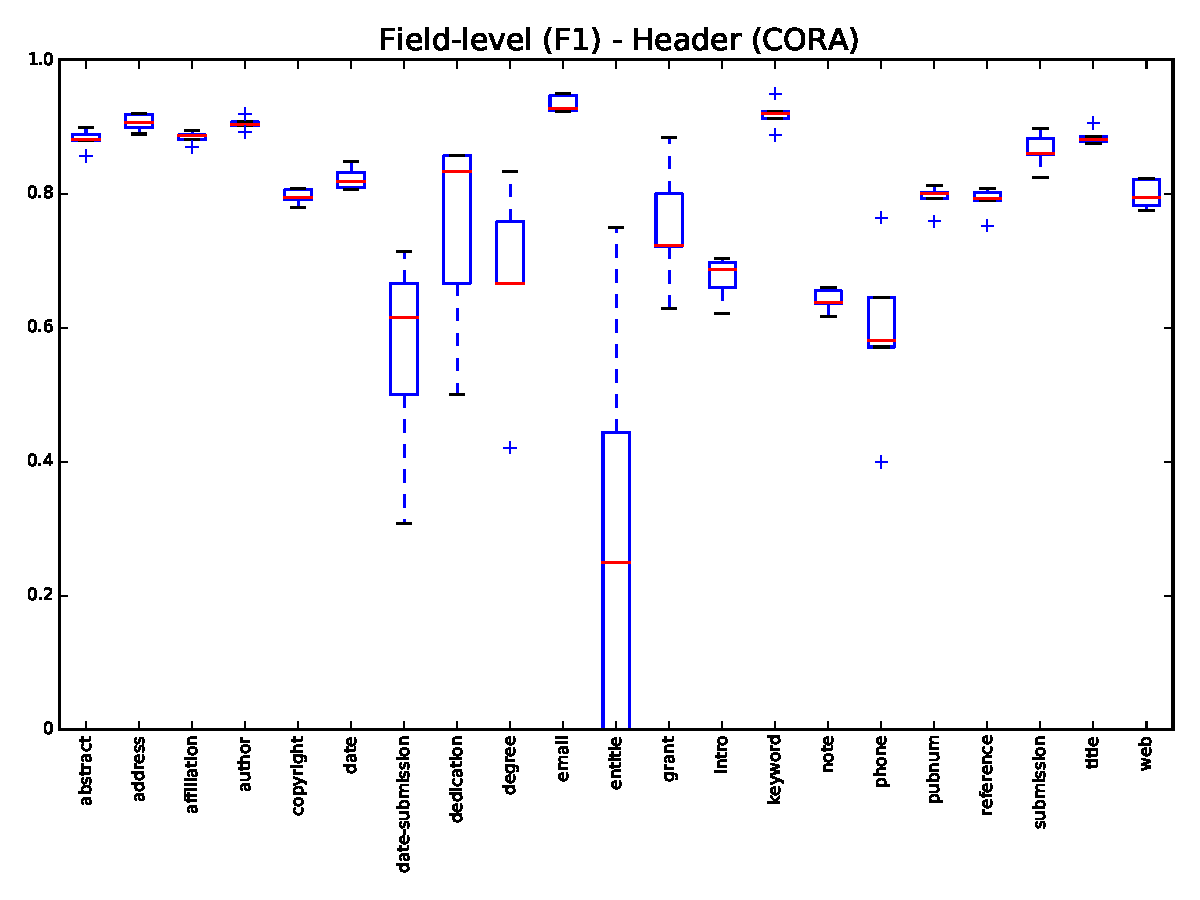
\includegraphics[width=0.75\textwidth]{../../figs/baseline/H_C/boxplot-field-level.pdf}}\\
%   \subfloat[][]{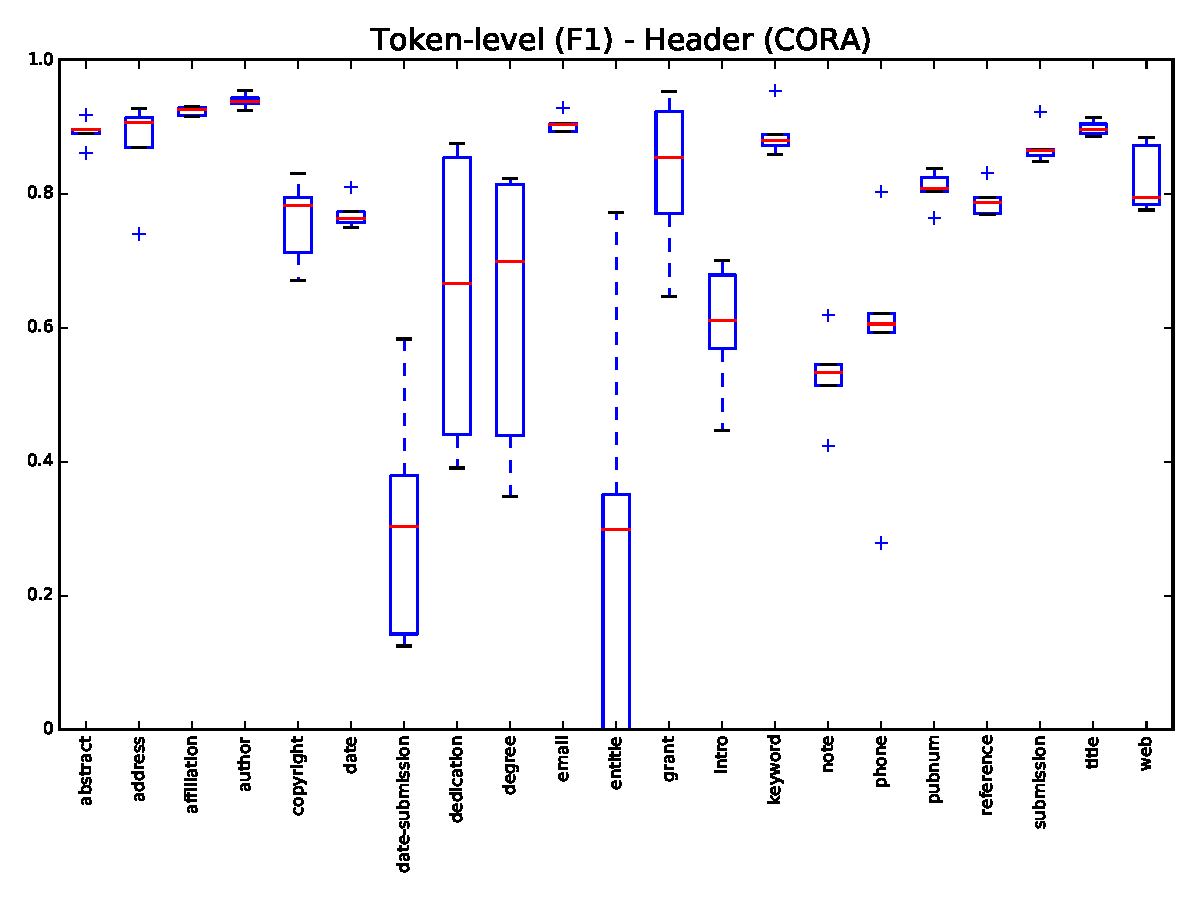
\includegraphics[width=0.75\textwidth]{../../figs/baseline/H_C/boxplot-token-level.pdf}}
% \end{figure}

% \begin{figure}[H]
%   \centering
%   \subfloat[][]{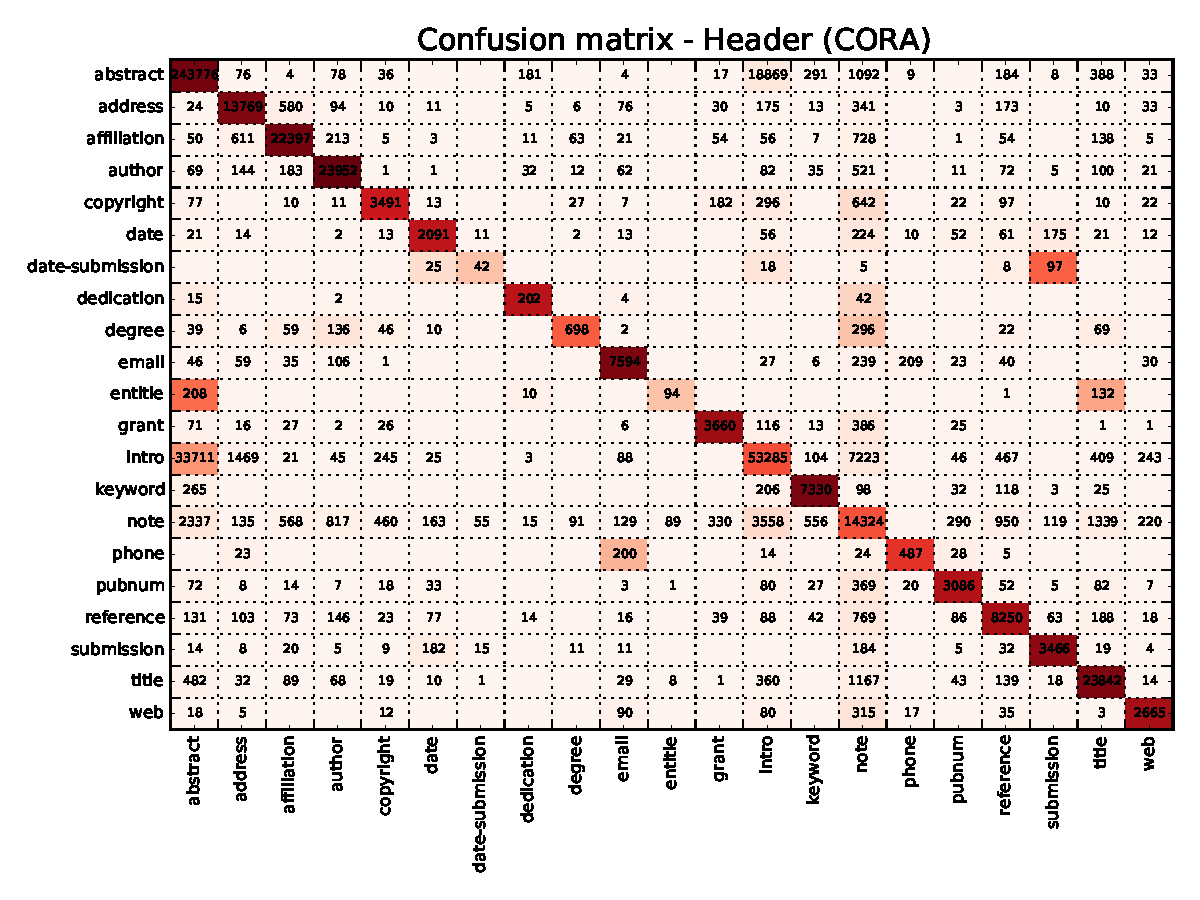
\includegraphics[width=0.75\textwidth]{../../figs/baseline/H_C/confusion_totals.pdf}}
% \end{figure}

% %%%%%%%%%%%%%%%%%%%%%%%%%%%%%%%%%%%%%%%%%%%%%%

% \subsubsection{Header model - Cora dataset appending HEP dataset}

% %%%%%%%%%%%%%%%%%%%%%%%%%%%%%%%%%%%%%%%%%%%%%%

% \begin{figure}[H]
%   \centering
%   \subfloat[][]{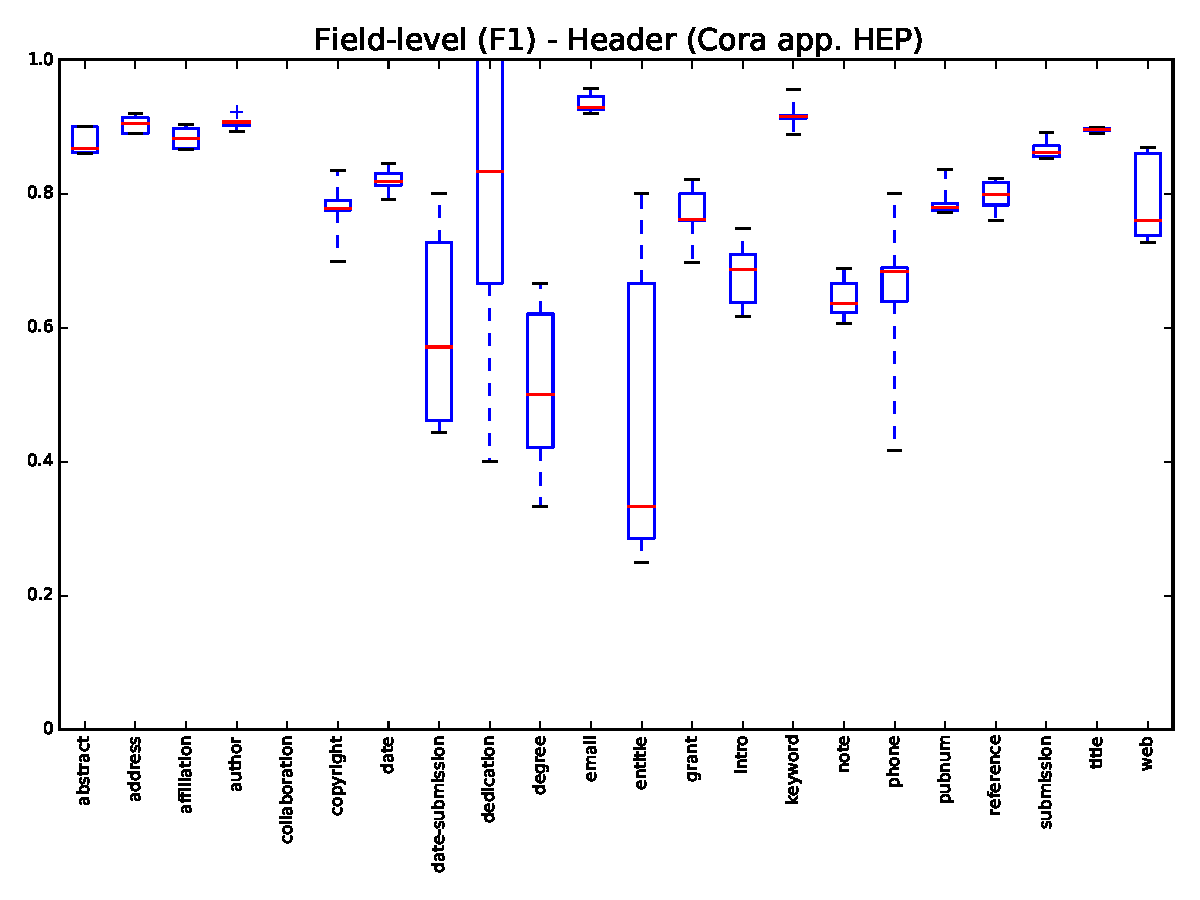
\includegraphics[width=0.75\textwidth]{../../figs/baseline/H_CappH/boxplot-field-level.pdf}}\\
%   \subfloat[][]{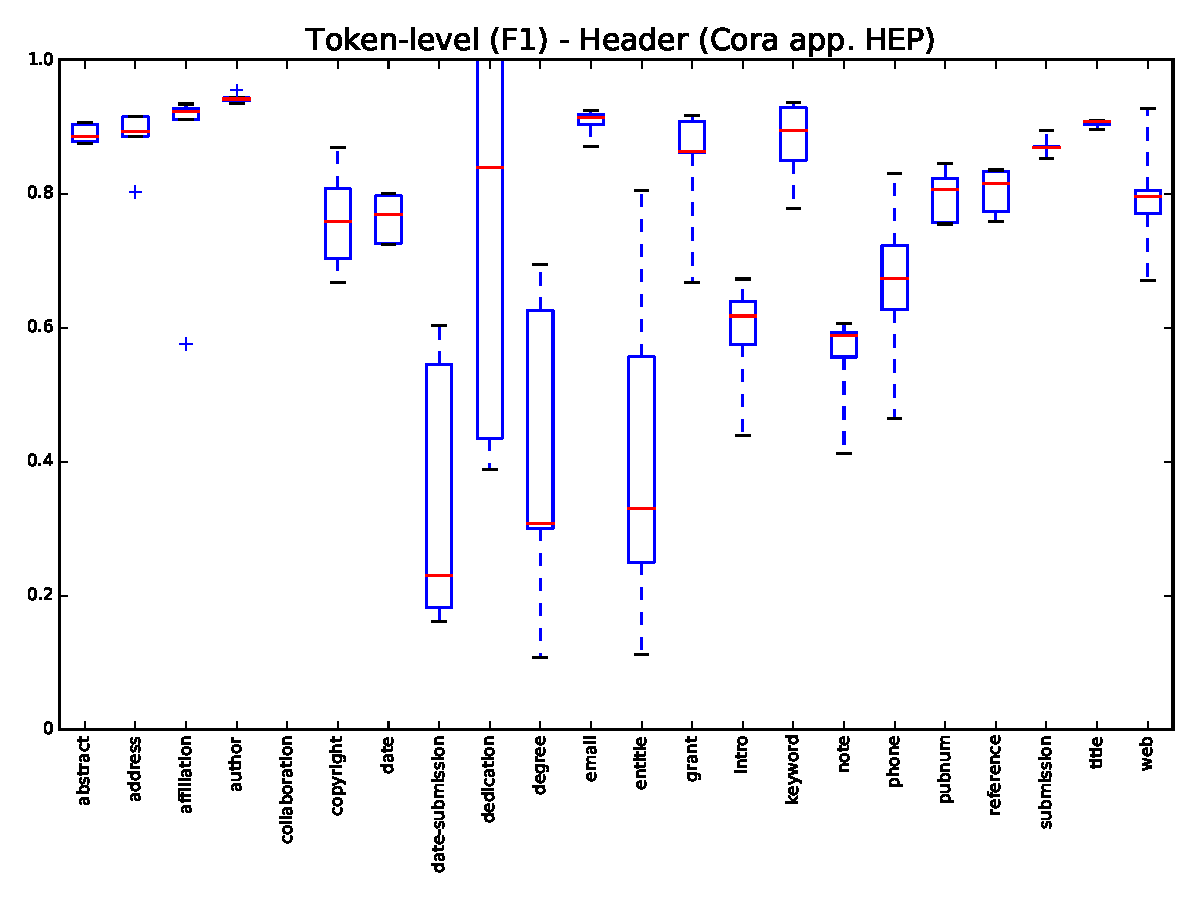
\includegraphics[width=0.75\textwidth]{../../figs/baseline/H_CappH/boxplot-token-level.pdf}}
% \end{figure}

% \begin{figure}[H]
%   \centering
%   \subfloat[][]{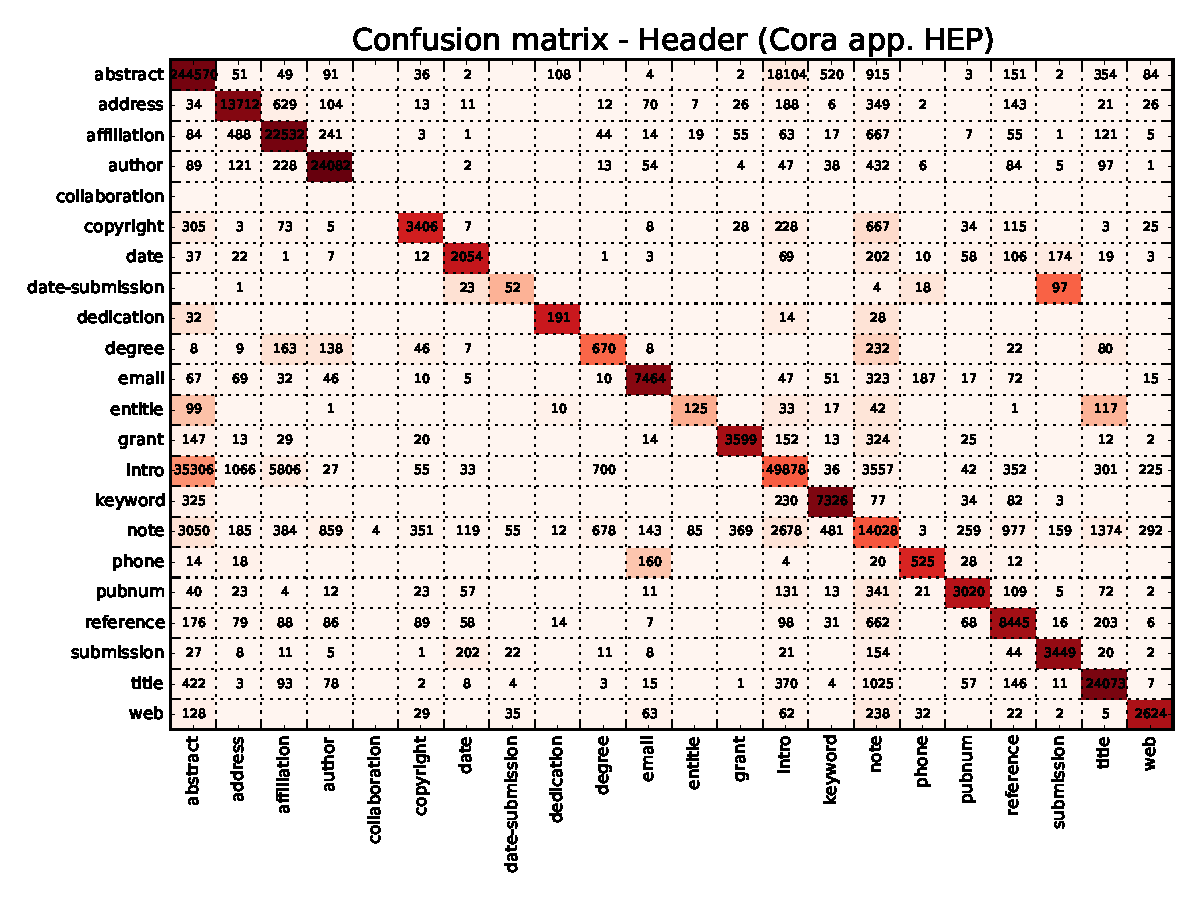
\includegraphics[width=0.75\textwidth]{../../figs/baseline/H_CappH/confusion_totals.pdf}}
% \end{figure}

% %%%%%%%%%%%%%%%%%%%%%%%%%%%%%%%%%%%%%%%%%%%%%%

% \subsubsection{Header model - Cora and HEP combined datasets}

% %%%%%%%%%%%%%%%%%%%%%%%%%%%%%%%%%%%%%%%%%%%%%%

% \begin{figure}[H]
%   \centering
%   \subfloat[][]{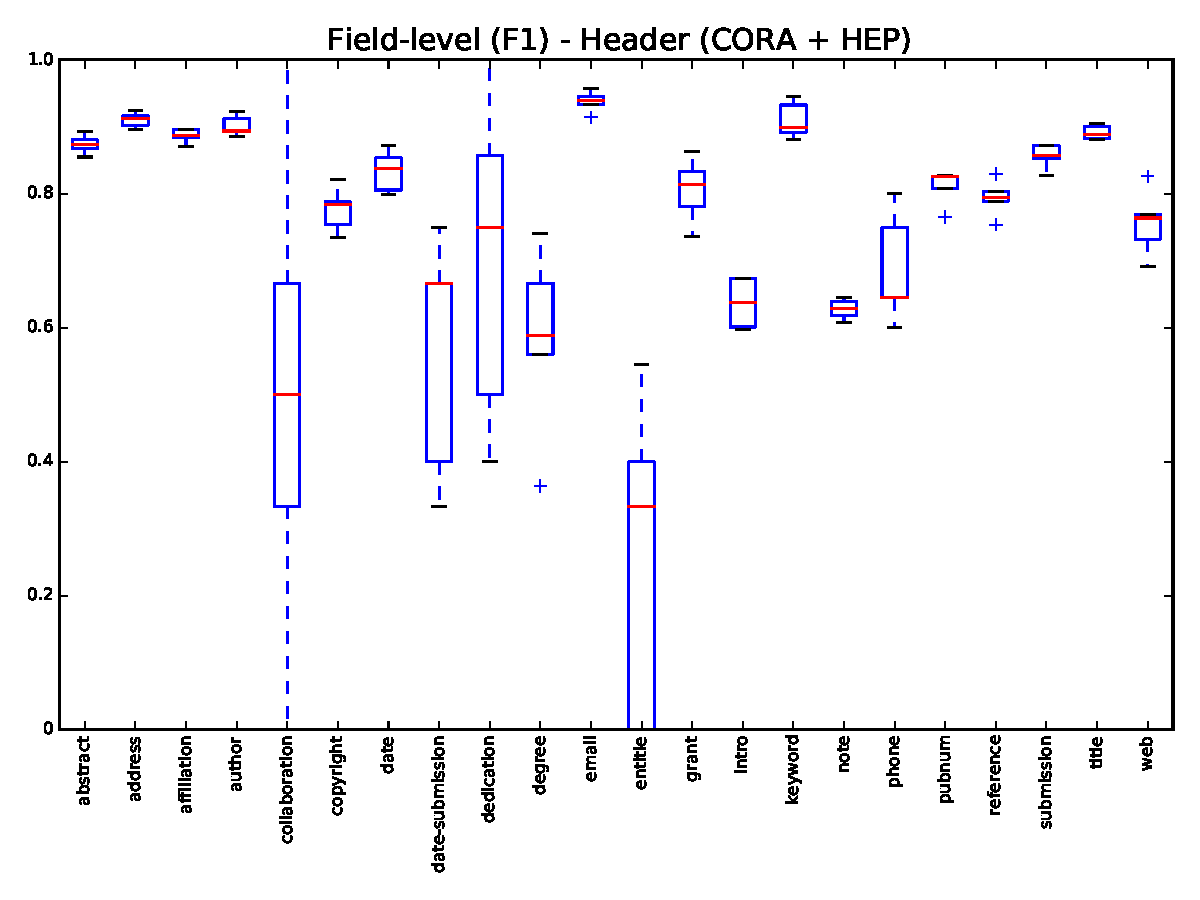
\includegraphics[width=0.75\textwidth]{../../figs/baseline/H_CH/boxplot-field-level.pdf}}\\
%   \subfloat[][]{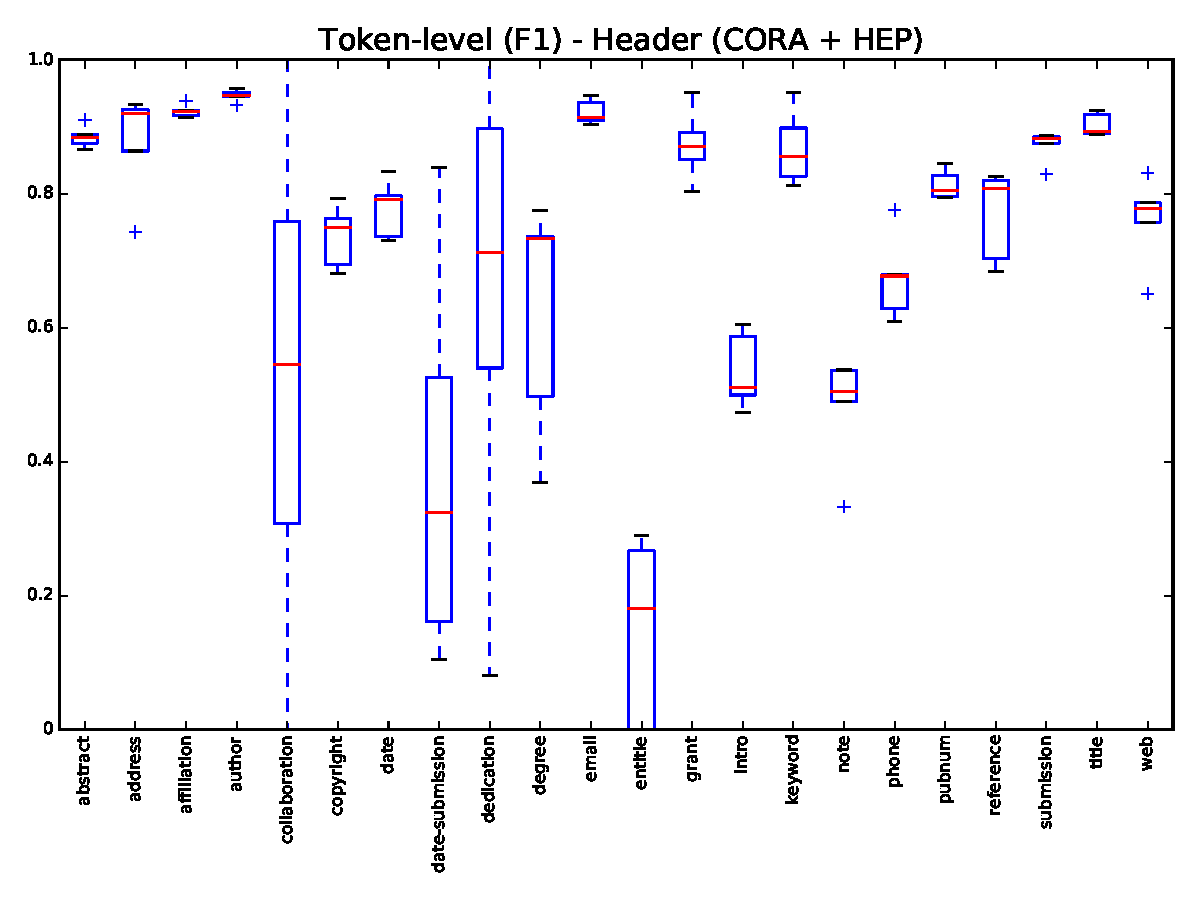
\includegraphics[width=0.75\textwidth]{../../figs/baseline/H_CH/boxplot-token-level.pdf}}
% \end{figure}

% \begin{figure}[H]
%   \centering
%   \subfloat[][]{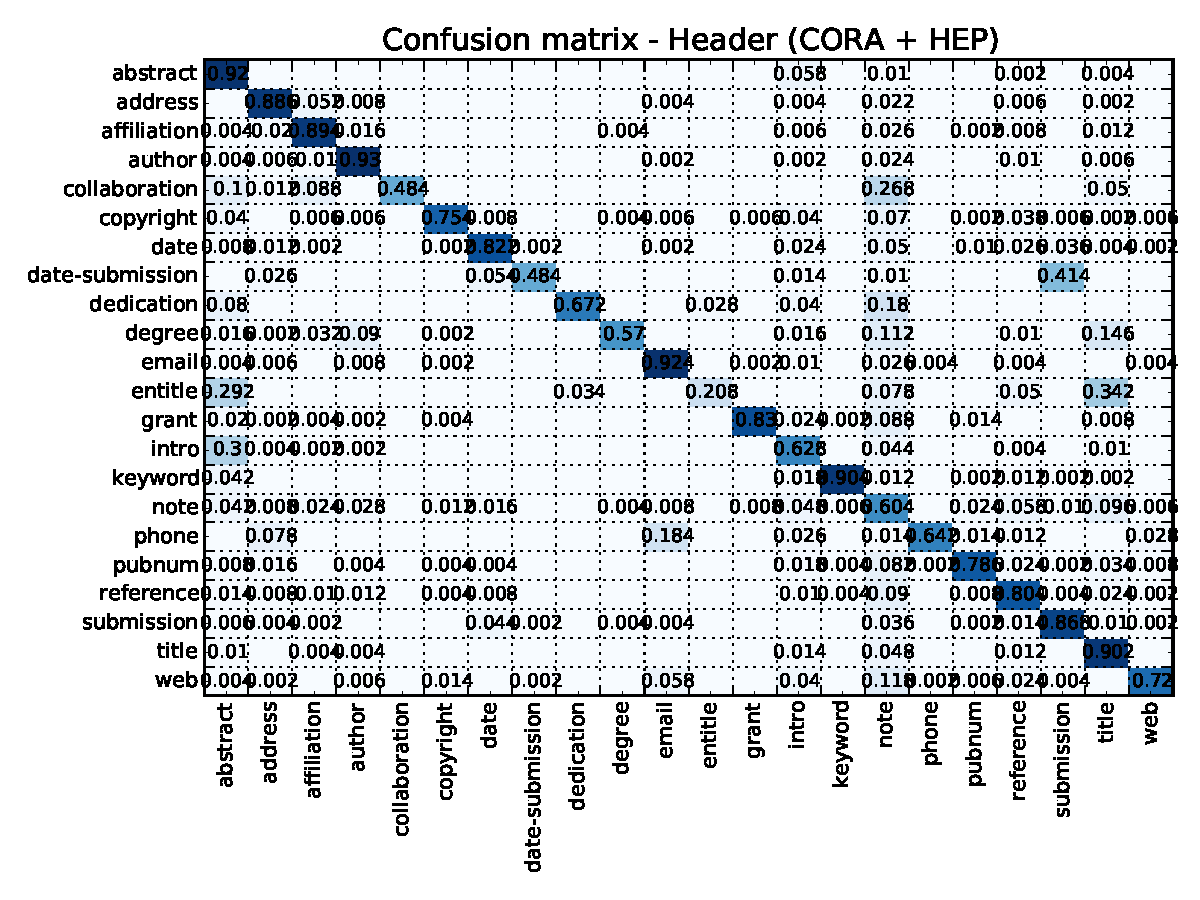
\includegraphics[width=0.75\textwidth]{../../figs/baseline/H_CH/confusion_averages.pdf}}\\
%   \subfloat[][]{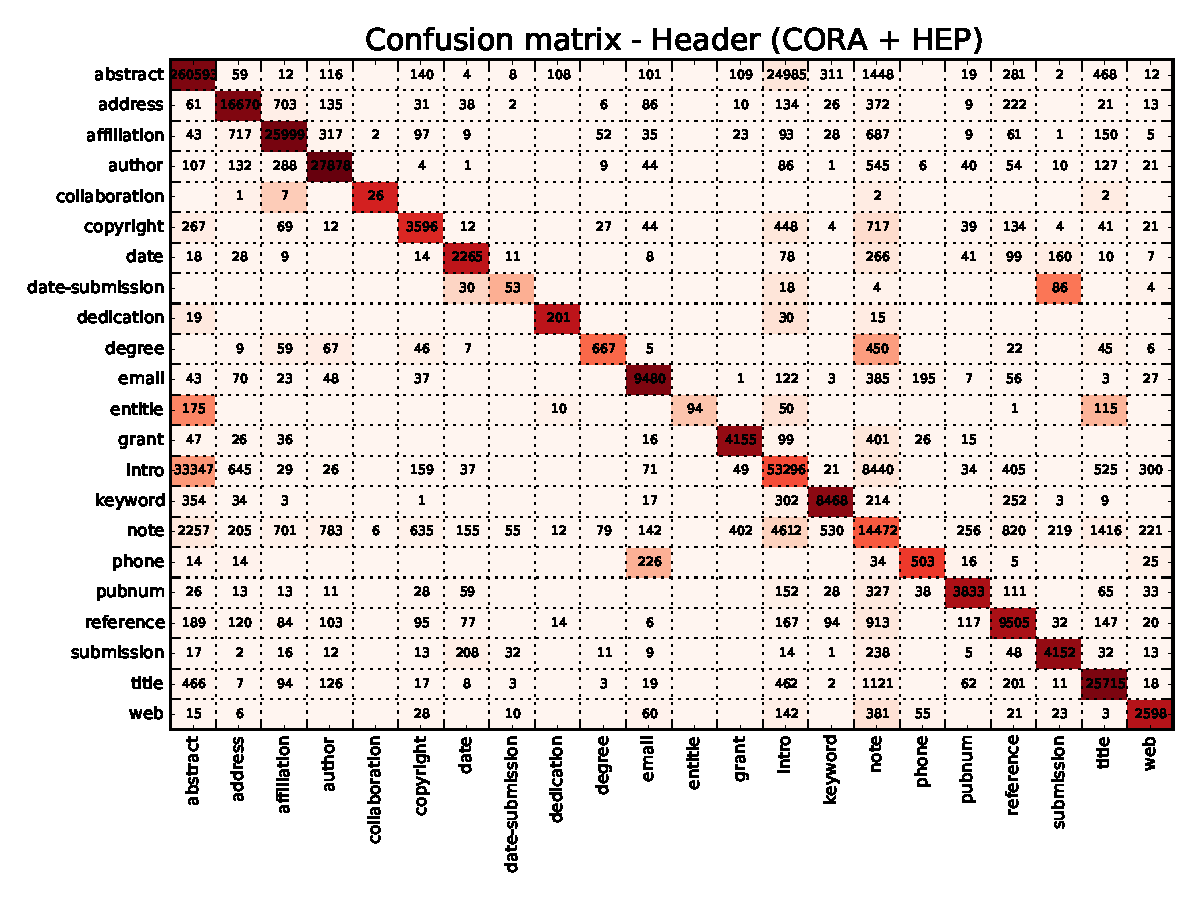
\includegraphics[width=0.75\textwidth]{../../figs/baseline/H_CH/confusion_totals.pdf}}
% \end{figure}

% %%%%%%%%%%%%%%%%%%%%%%%%%%%%%%%%%%%%%%%%%%%%%%

% \subsubsection{Header model - HEP dataset}

% %%%%%%%%%%%%%%%%%%%%%%%%%%%%%%%%%%%%%%%%%%%%%%

% \begin{figure}[H]
%   \centering
%   \subfloat[][]{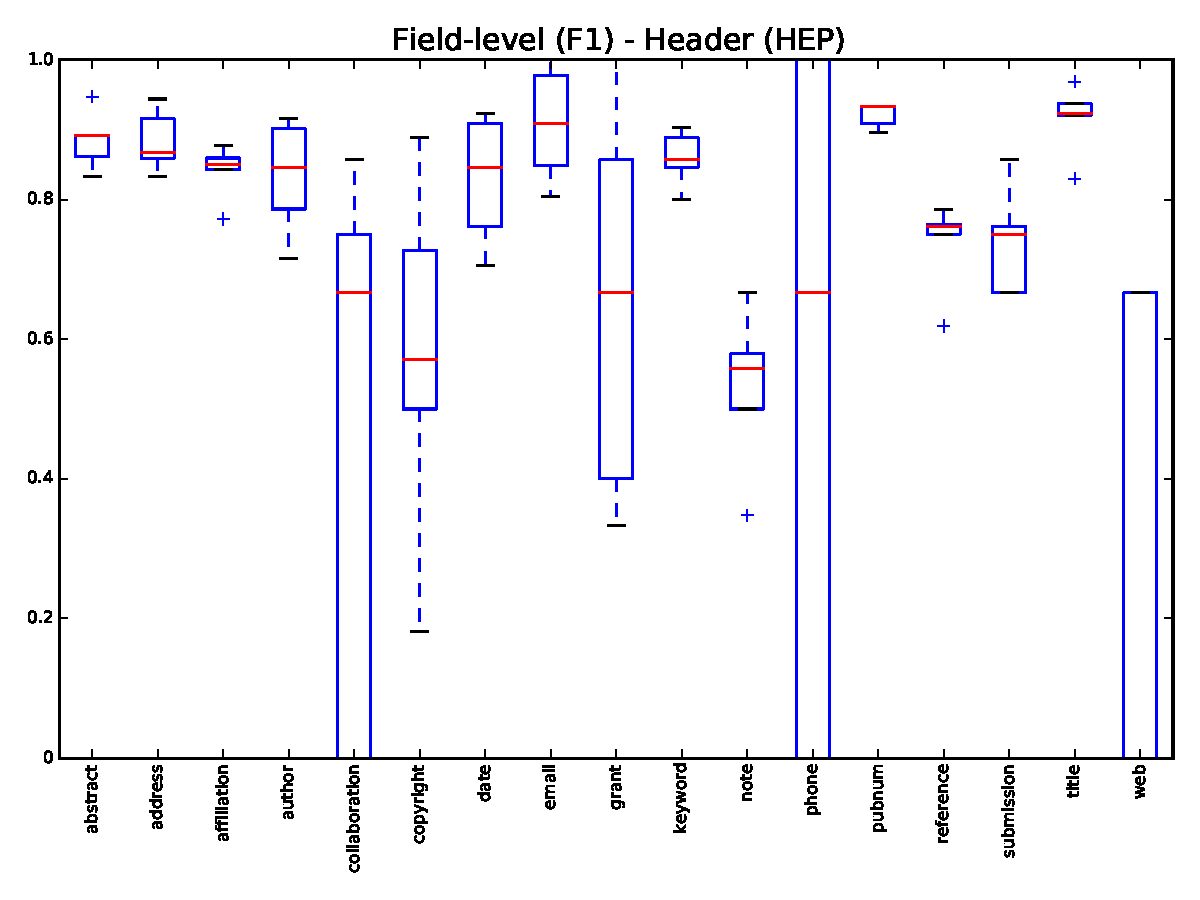
\includegraphics[width=0.75\textwidth]{../../figs/baseline/H_H/boxplot-field-level.pdf}}\\
%   \subfloat[][]{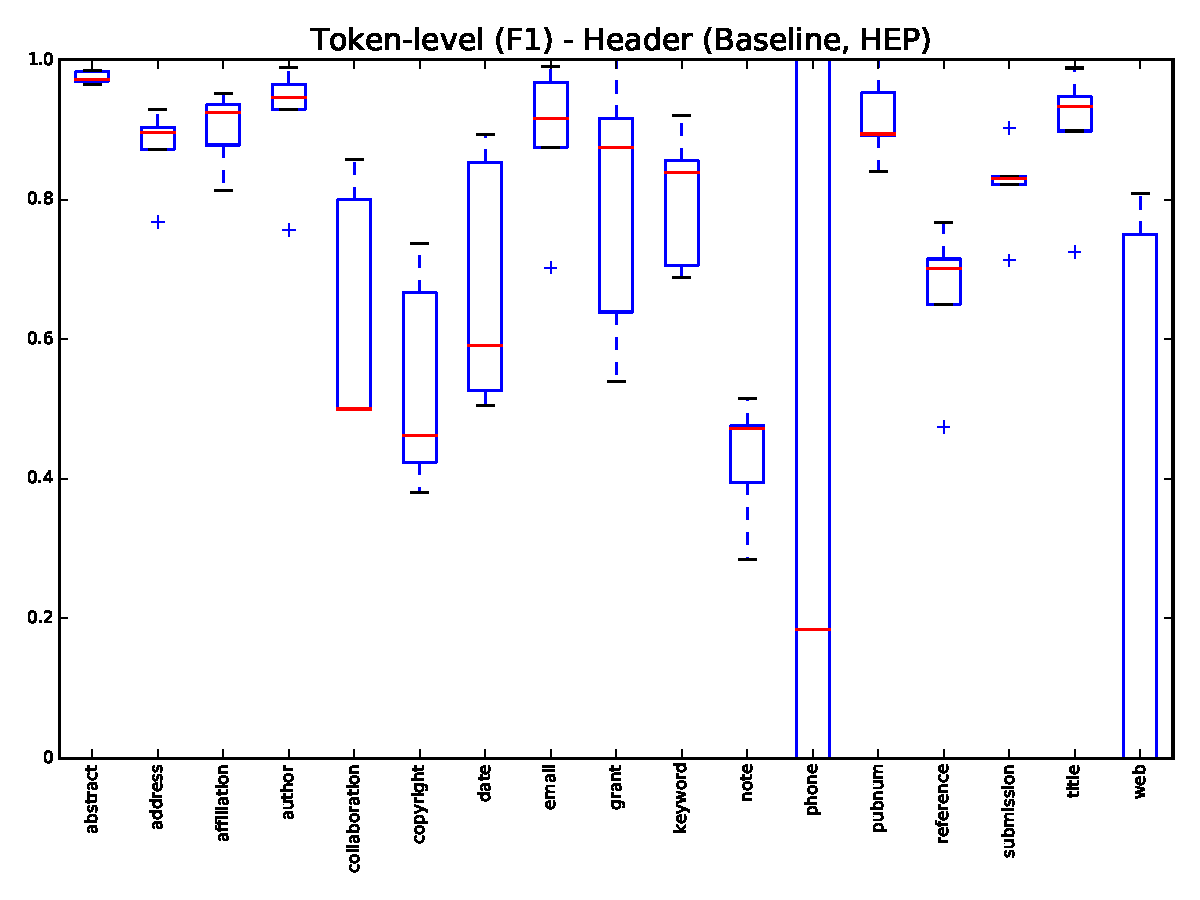
\includegraphics[width=0.75\textwidth]{../../figs/baseline/H_H/boxplot-token-level.pdf}}
% \end{figure}

% \begin{figure}[H]
%   \centering
%   \subfloat[][]{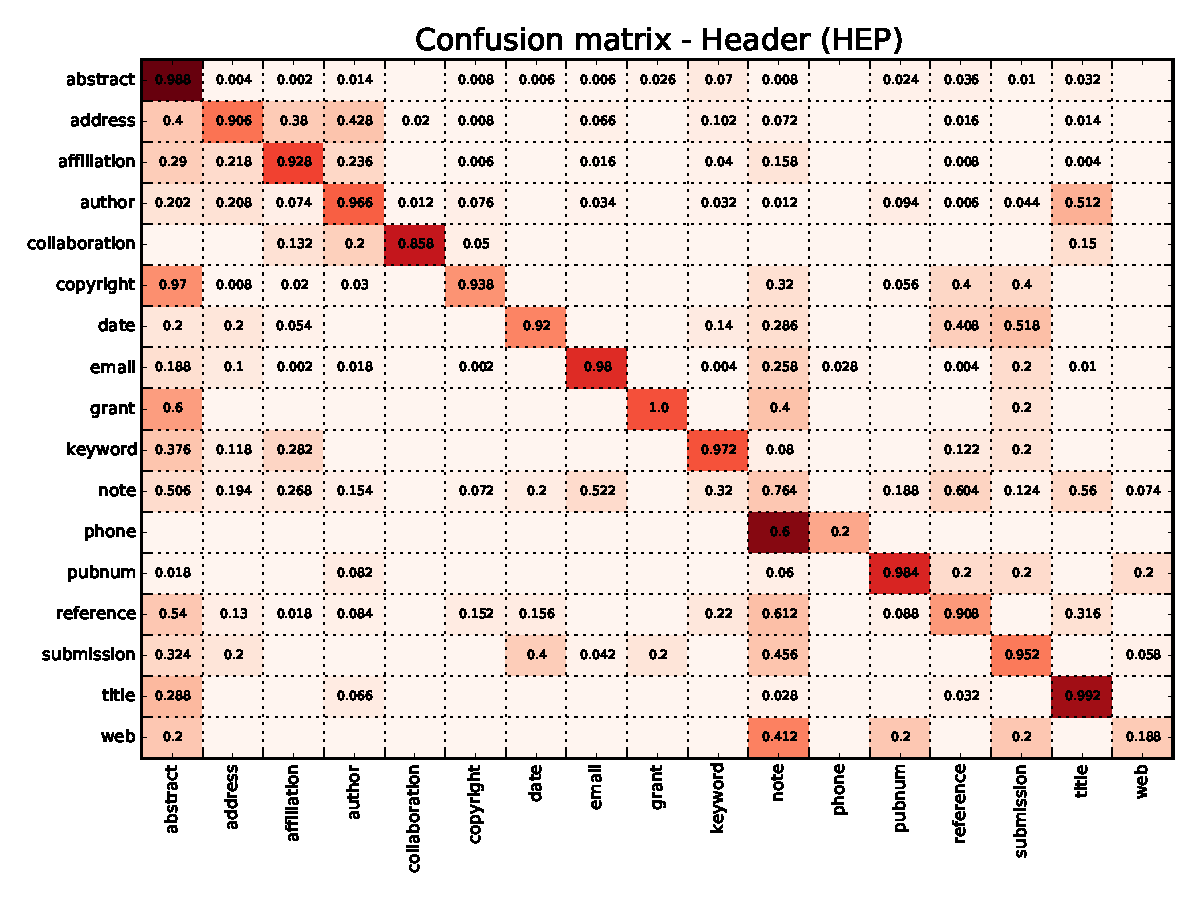
\includegraphics[width=0.75\textwidth]{../../figs/baseline/H_H/confusion_averages.pdf}}\\
%   \subfloat[][]{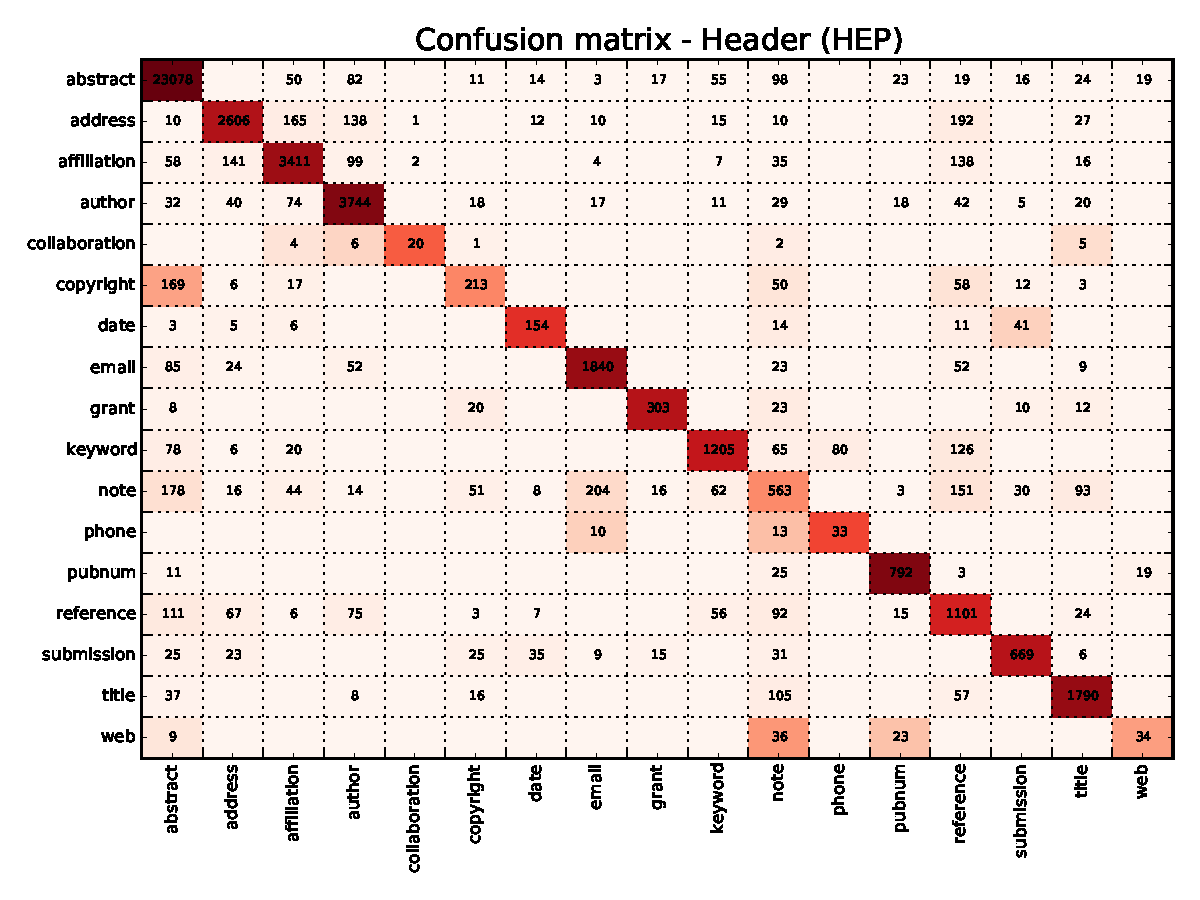
\includegraphics[width=0.75\textwidth]{../../figs/baseline/H_H/confusion_totals.pdf}}
% \end{figure}

% %%%%%%%%%%%%%%%%%%%%%%%%%%%%%%%%%%%%%%%%%%%%%%

% \subsubsection{Header model - HEP dataset appending CORA dataset}

% %%%%%%%%%%%%%%%%%%%%%%%%%%%%%%%%%%%%%%%%%%%%%%

% \begin{figure}[H]
%   \centering
%   \subfloat[][]{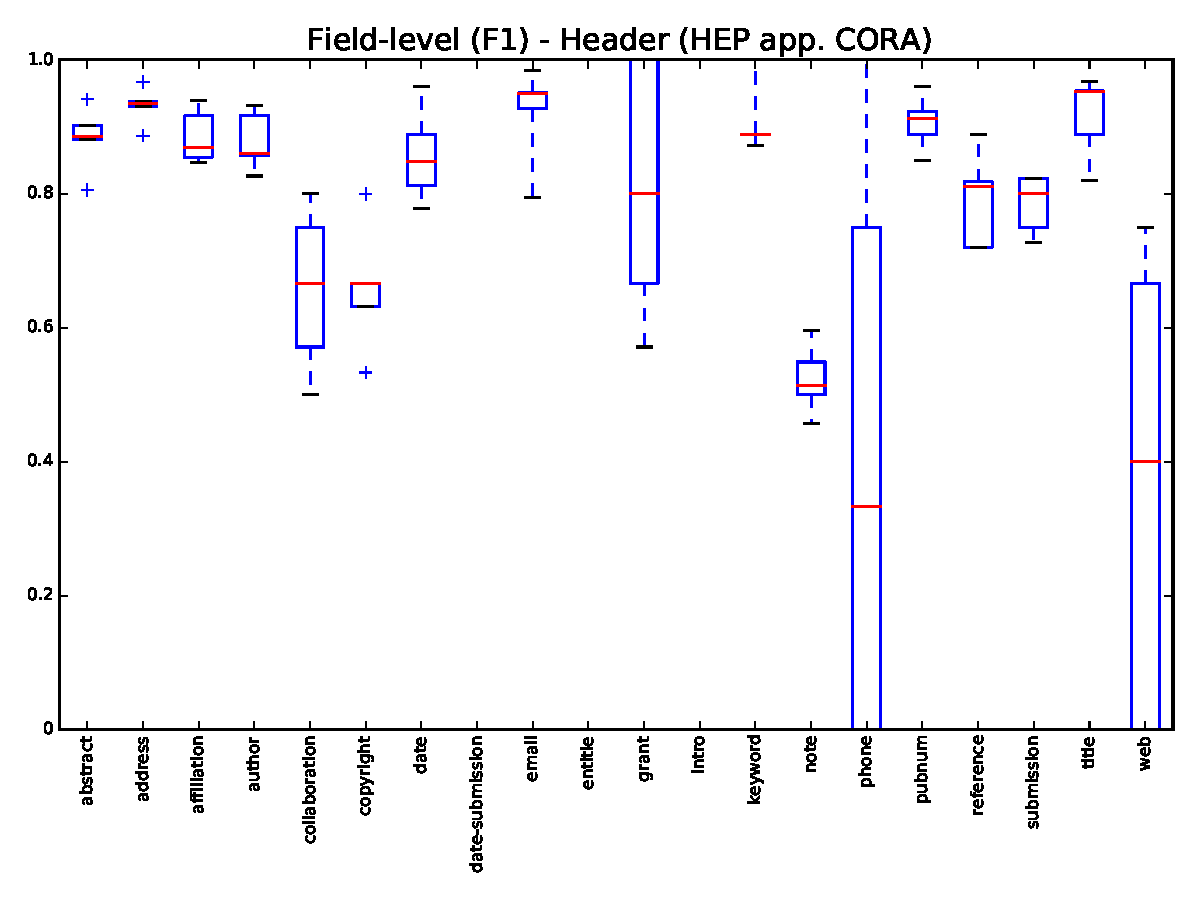
\includegraphics[width=0.75\textwidth]{../../figs/baseline/H_HappC/boxplot-field-level.pdf}}\\
%   \subfloat[][]{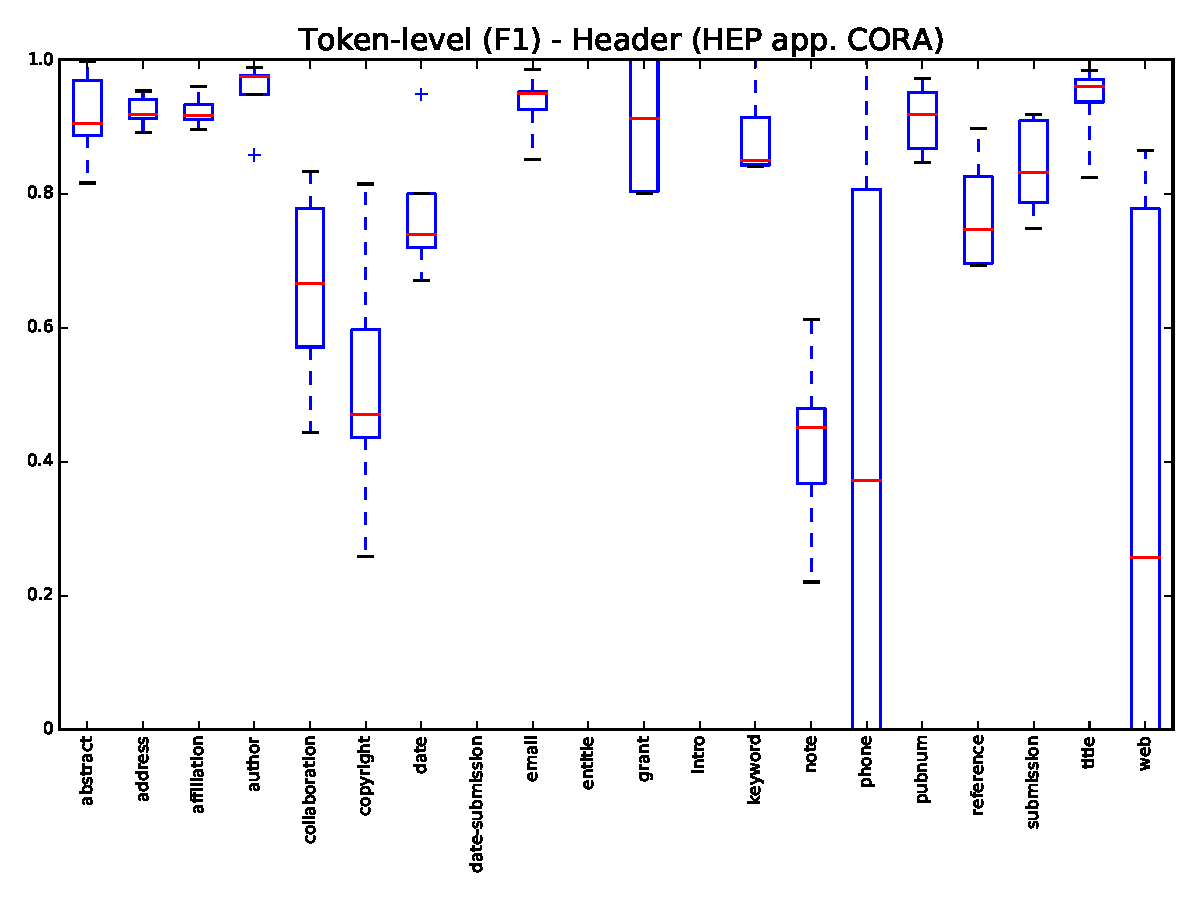
\includegraphics[width=0.75\textwidth]{../../figs/baseline/H_HappC/boxplot-token-level.pdf}}
% \end{figure}

% \begin{figure}[H]
%   \centering
%   \subfloat[][]{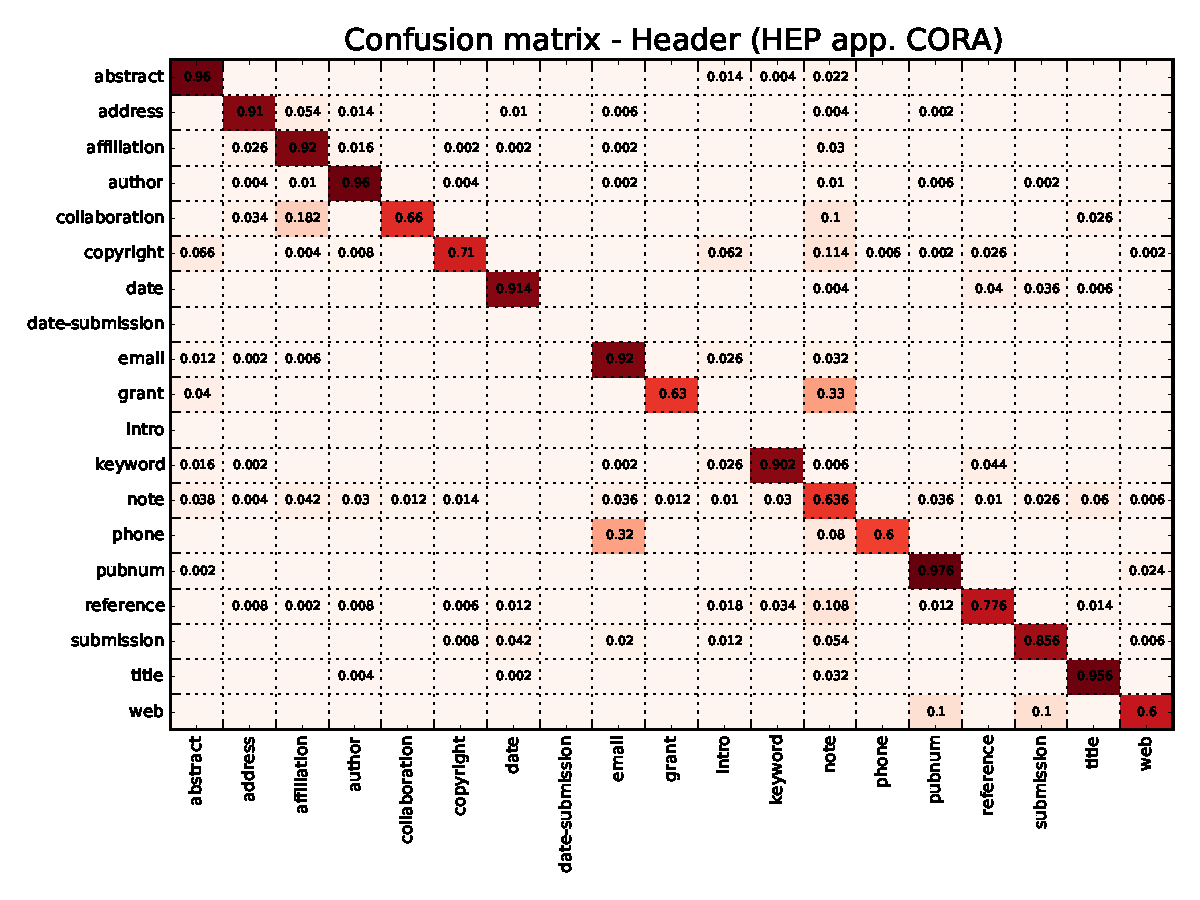
\includegraphics[width=0.75\textwidth]{../../figs/baseline/H_HappC/confusion_averages.pdf}}\\
%   \subfloat[][]{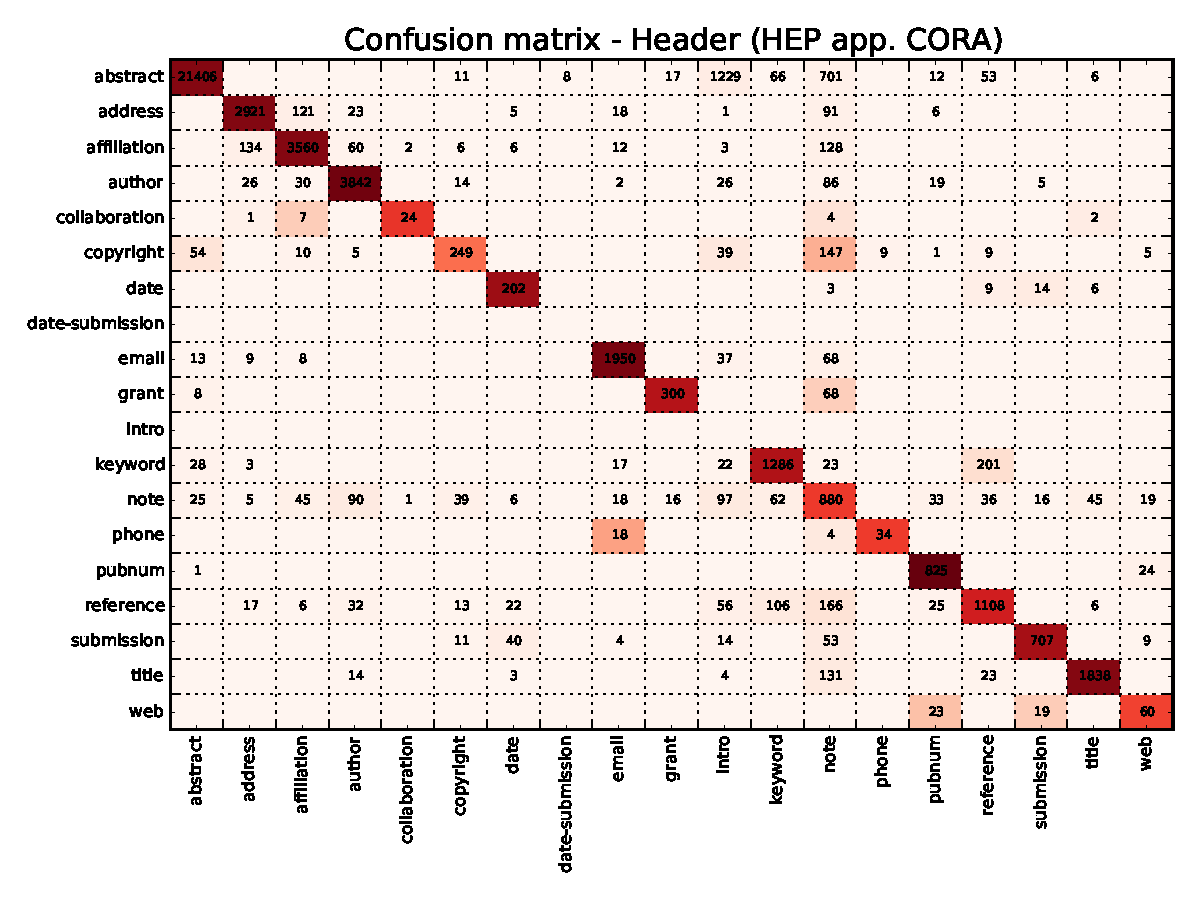
\includegraphics[width=0.75\textwidth]{../../figs/baseline/H_HappC/confusion_totals.pdf}}
% \end{figure}

% %%%%%%%%%%%%%%%%%%%%%%%%%%%%%%%%%%%%%%%%%%%%%%

% \subsubsection{Header model - HEP dataset appending 1/3 CORA dataset}

% %%%%%%%%%%%%%%%%%%%%%%%%%%%%%%%%%%%%%%%%%%%%%%

% \begin{figure}[H]
%   \centering
%   \subfloat[][]{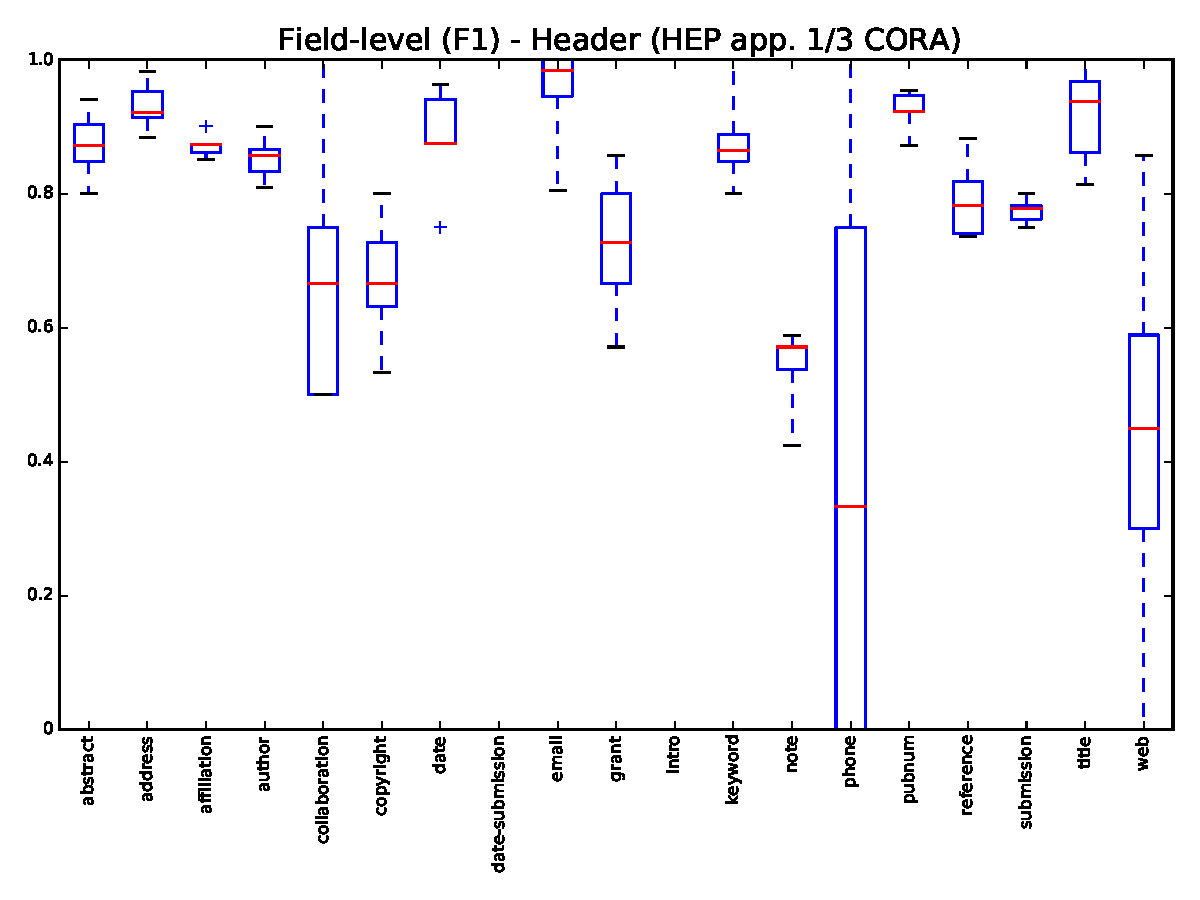
\includegraphics[width=0.75\textwidth]{../../figs/baseline/H_HappC333/boxplot-field-level.pdf}}\\
%   \subfloat[][]{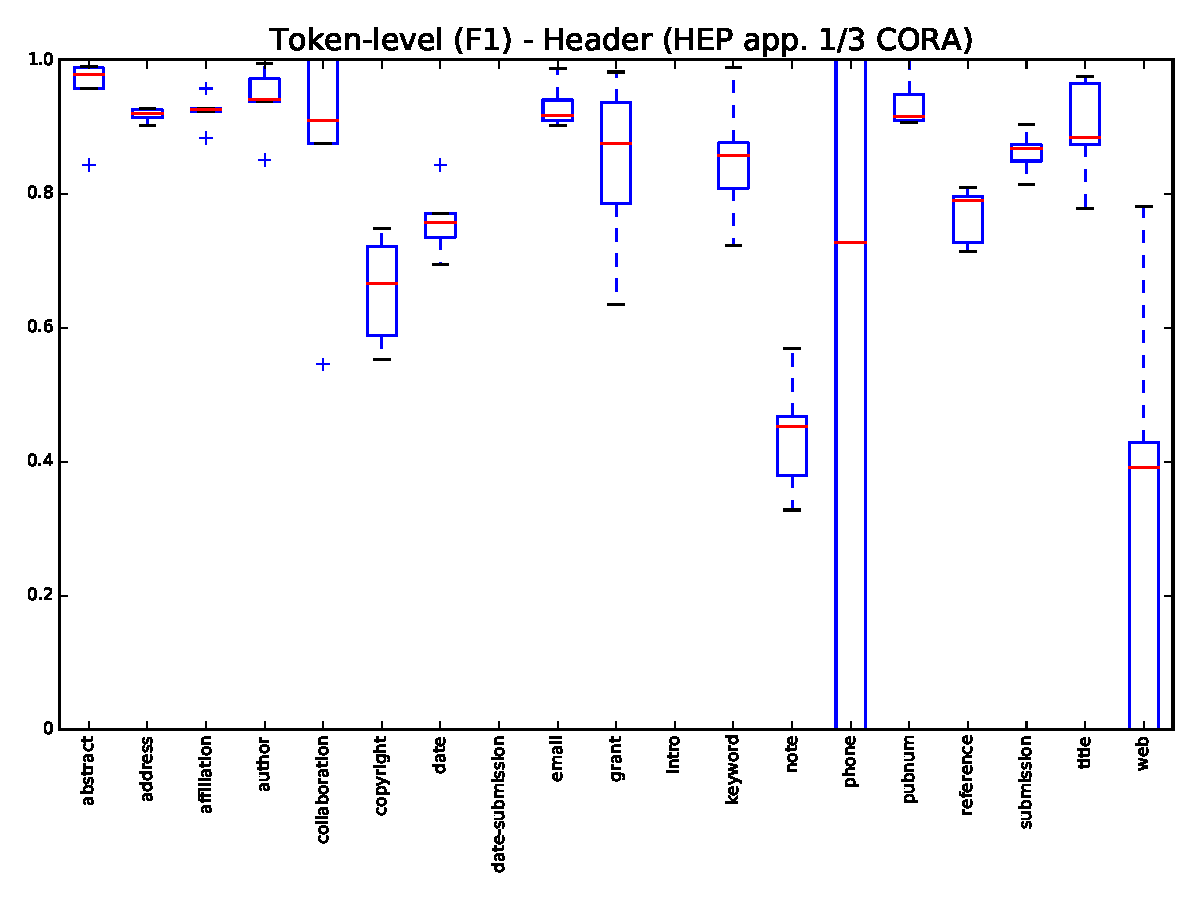
\includegraphics[width=0.75\textwidth]{../../figs/baseline/H_HappC333/boxplot-token-level.pdf}}
% \end{figure}

% \begin{figure}[H]
%   \centering
%   \subfloat[][]{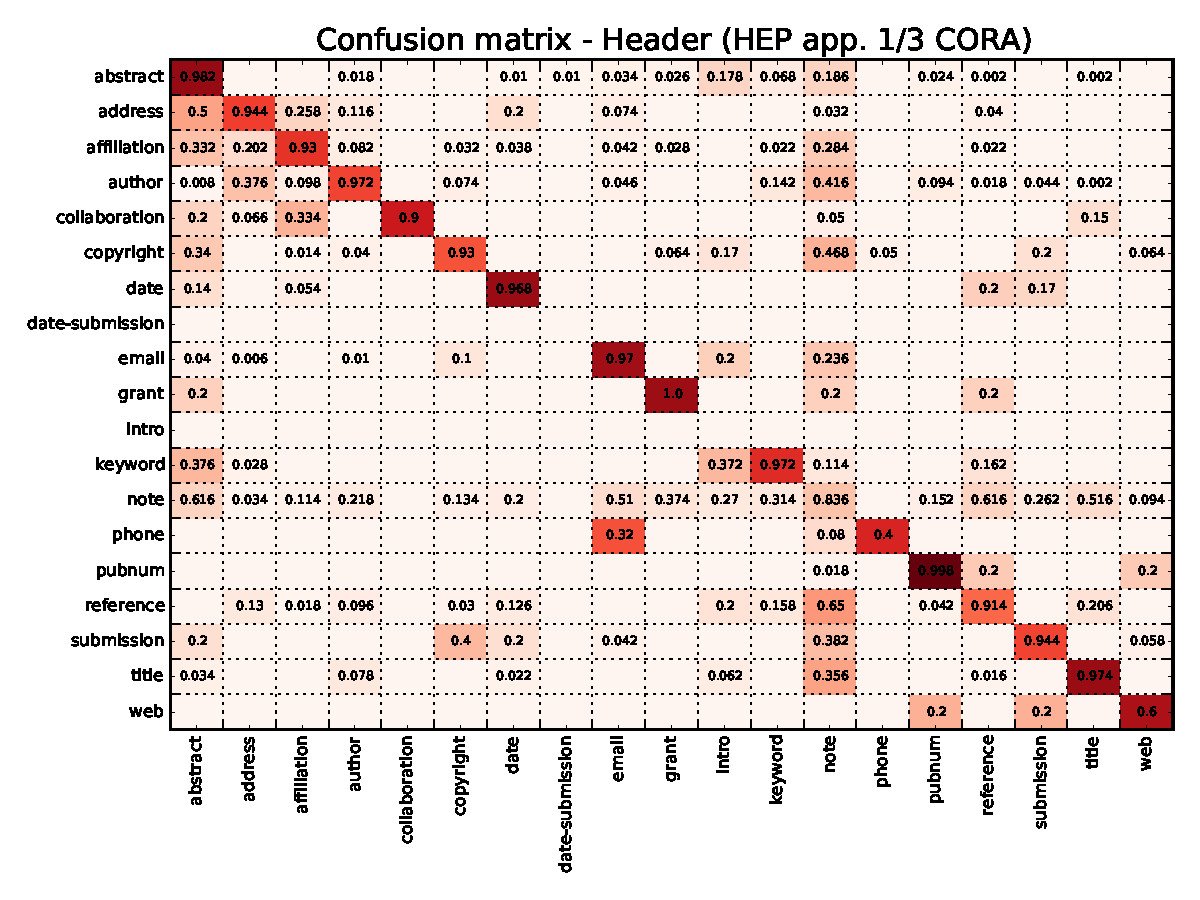
\includegraphics[width=0.75\textwidth]{../../figs/baseline/H_HappC333/confusion_averages.pdf}}\\
%   \subfloat[][]{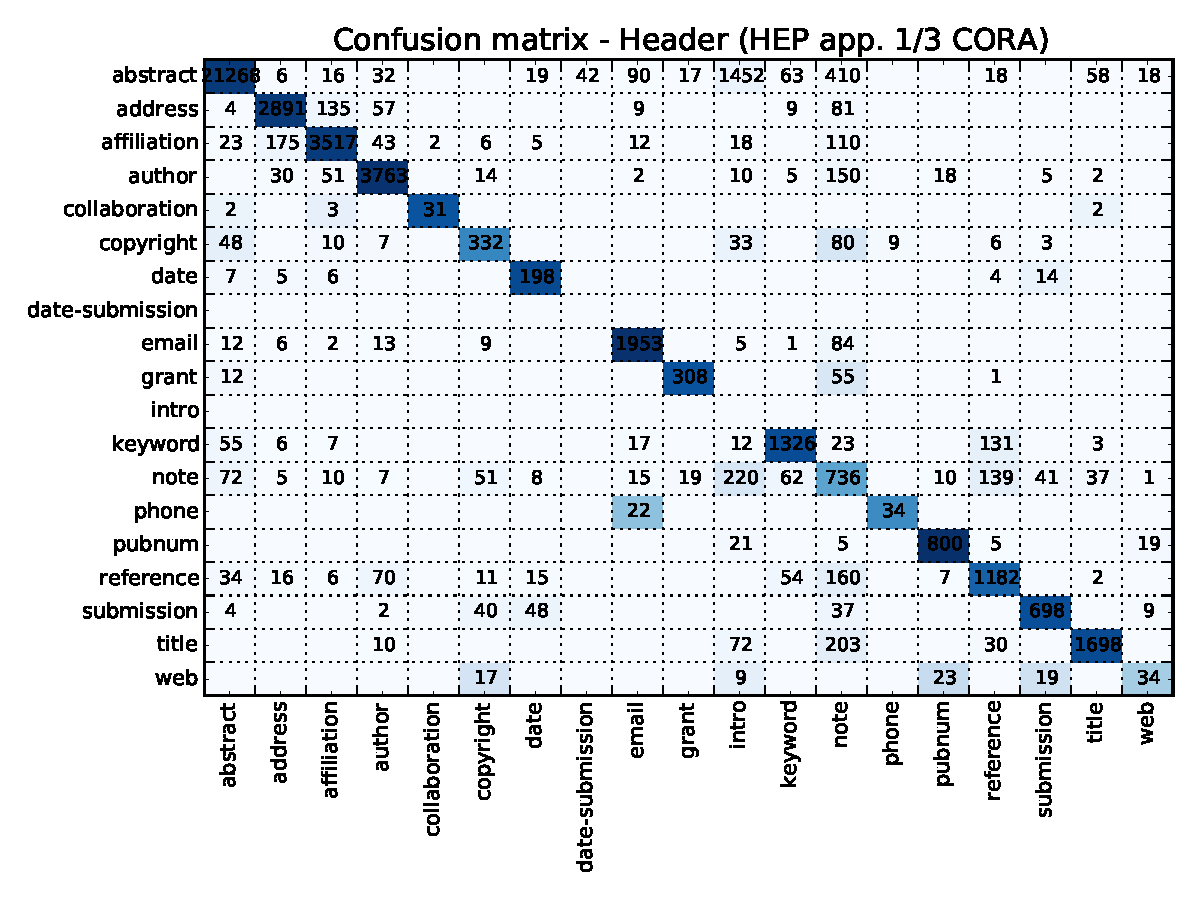
\includegraphics[width=0.75\textwidth]{../../figs/baseline/H_HappC333/confusion_totals.pdf}}
% \end{figure}

% %%%%%%%%%%%%%%%%%%%%%%%%%%%%%%%%%%%%%%%%%%%%%%

% \subsubsection{Header model - HEP dataset appending 2/3 CORA dataset}

% %%%%%%%%%%%%%%%%%%%%%%%%%%%%%%%%%%%%%%%%%%%%%%

% \begin{figure}[H]
%   \centering
%   \subfloat[][]{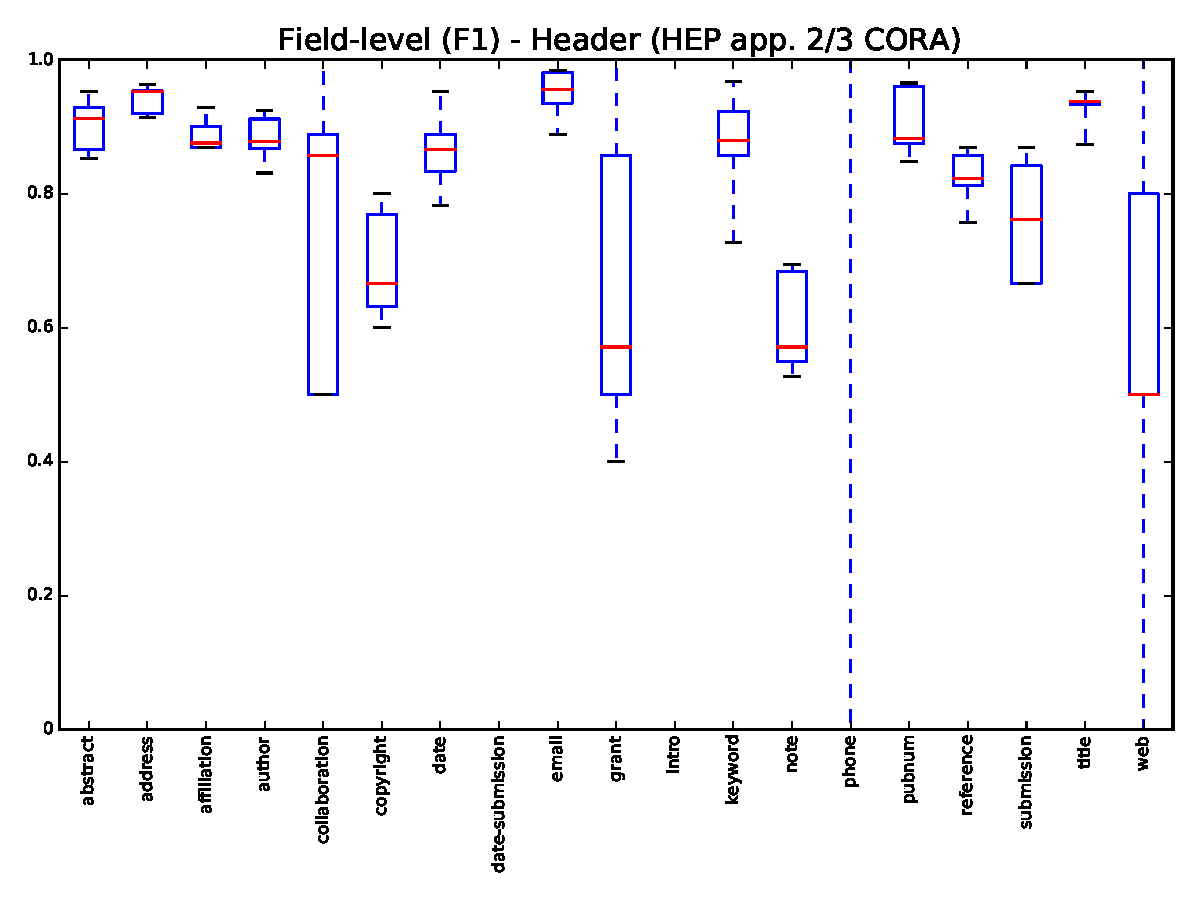
\includegraphics[width=0.75\textwidth]{../../figs/baseline/H_HappC666/boxplot-field-level.pdf}}\\
%   \subfloat[][]{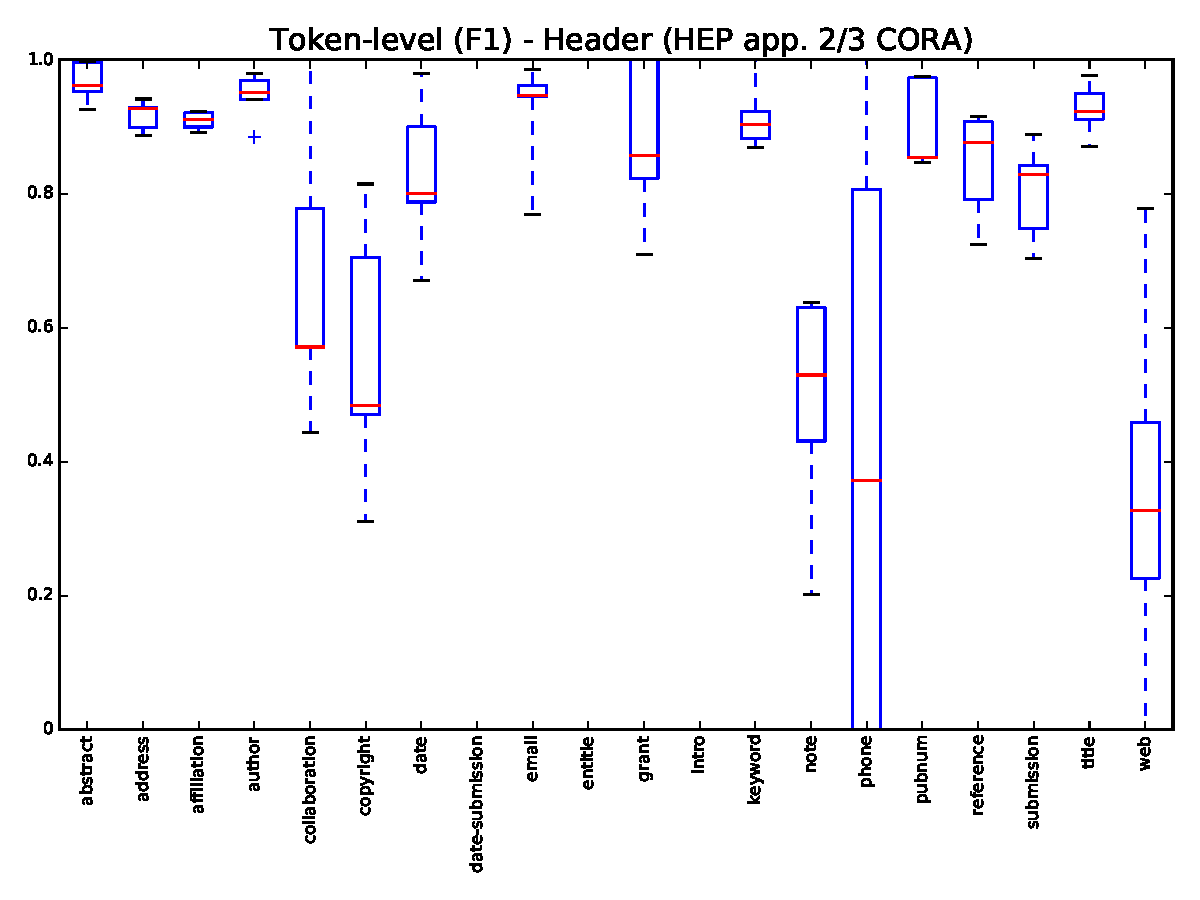
\includegraphics[width=0.75\textwidth]{../../figs/baseline/H_HappC666/boxplot-token-level.pdf}}
% \end{figure}

% \begin{figure}[H]
%   \centering
%   \subfloat[][]{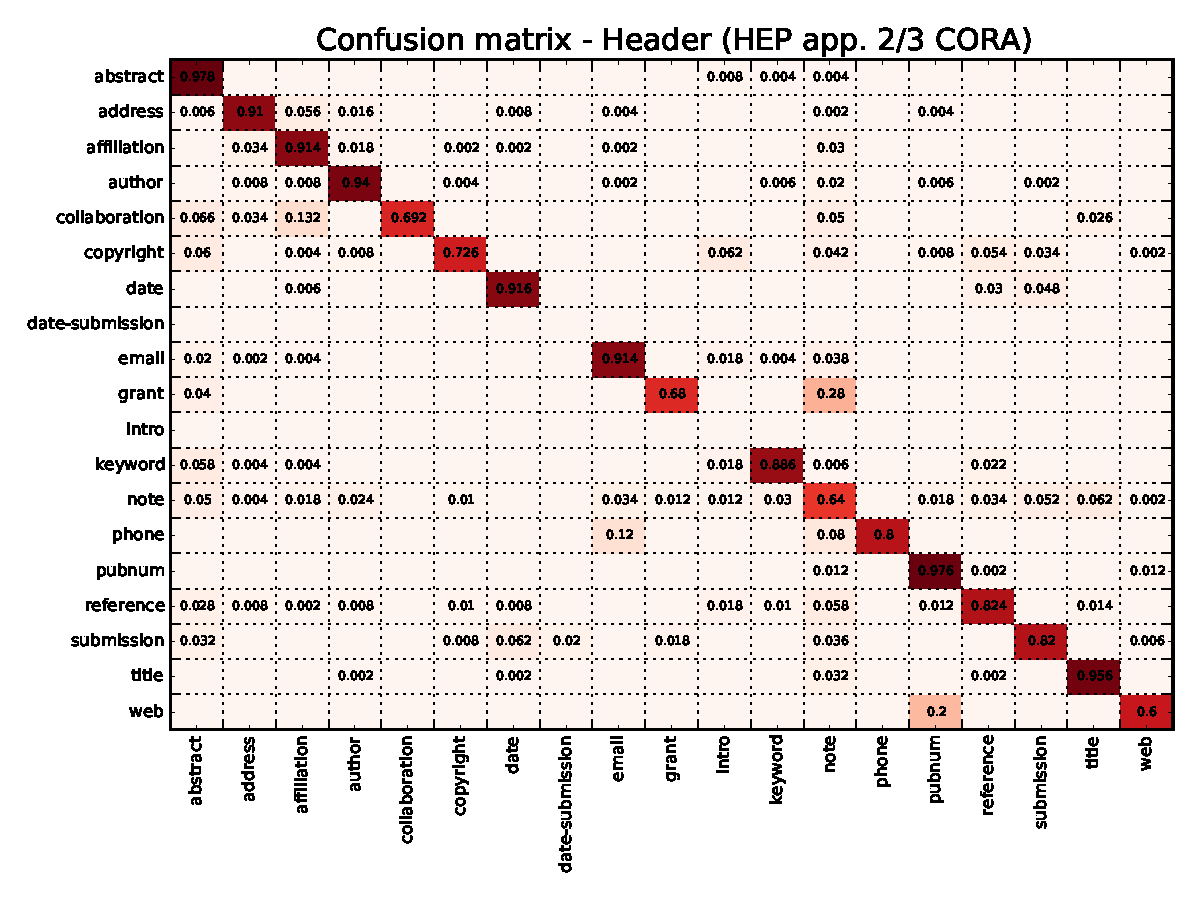
\includegraphics[width=0.75\textwidth]{../../figs/baseline/H_HappC666/confusion_averages.pdf}}\\
%   \subfloat[][]{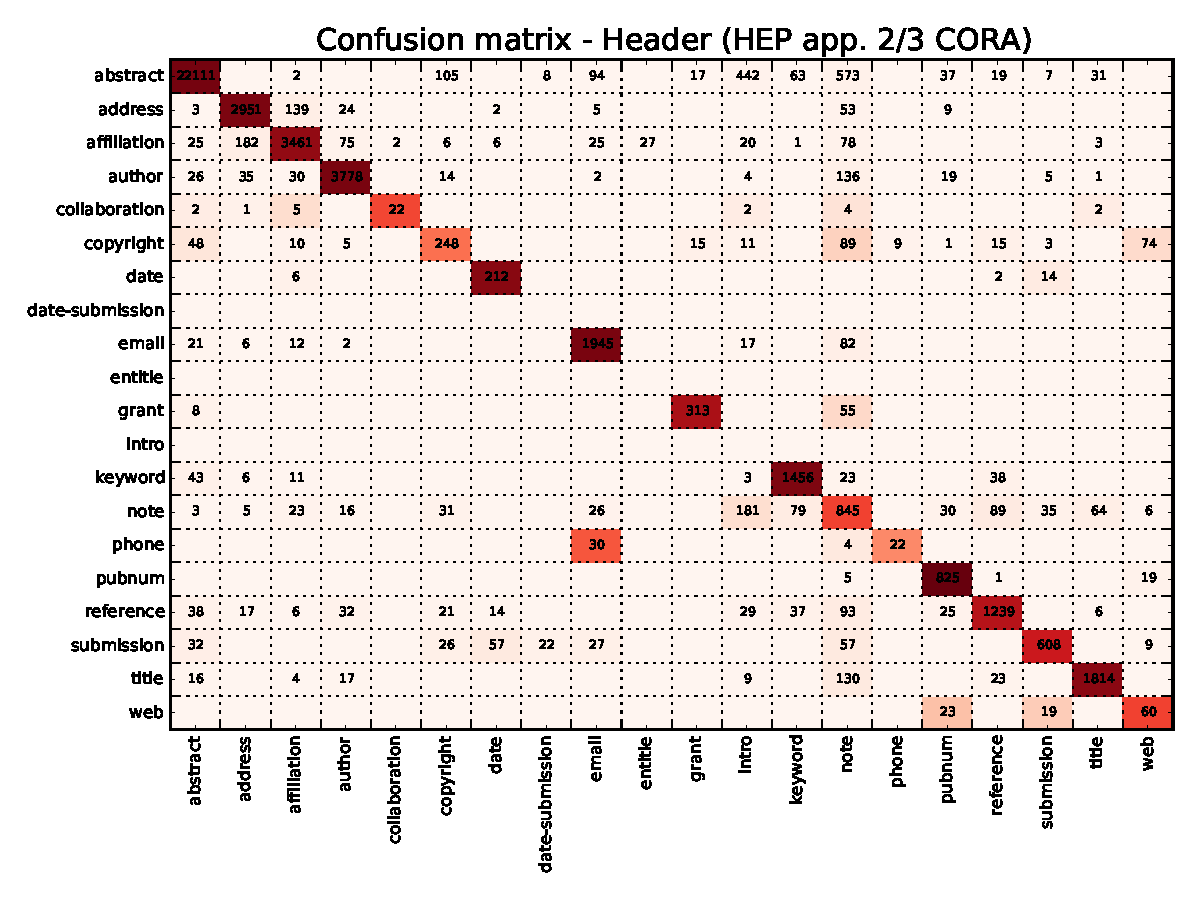
\includegraphics[width=0.75\textwidth]{../../figs/baseline/H_HappC666/confusion_totals.pdf}}
% \end{figure}

% %%%%%%%%%%%%%%%%%%%%%%%%%%%%%%%%%%%%%%%%%%%%%%

% \subsubsection{Segmentation model - Cora dataset}

% %%%%%%%%%%%%%%%%%%%%%%%%%%%%%%%%%%%%%%%%%%%%%%

% \begin{figure}[H]
%   \centering
%   \subfloat[][]{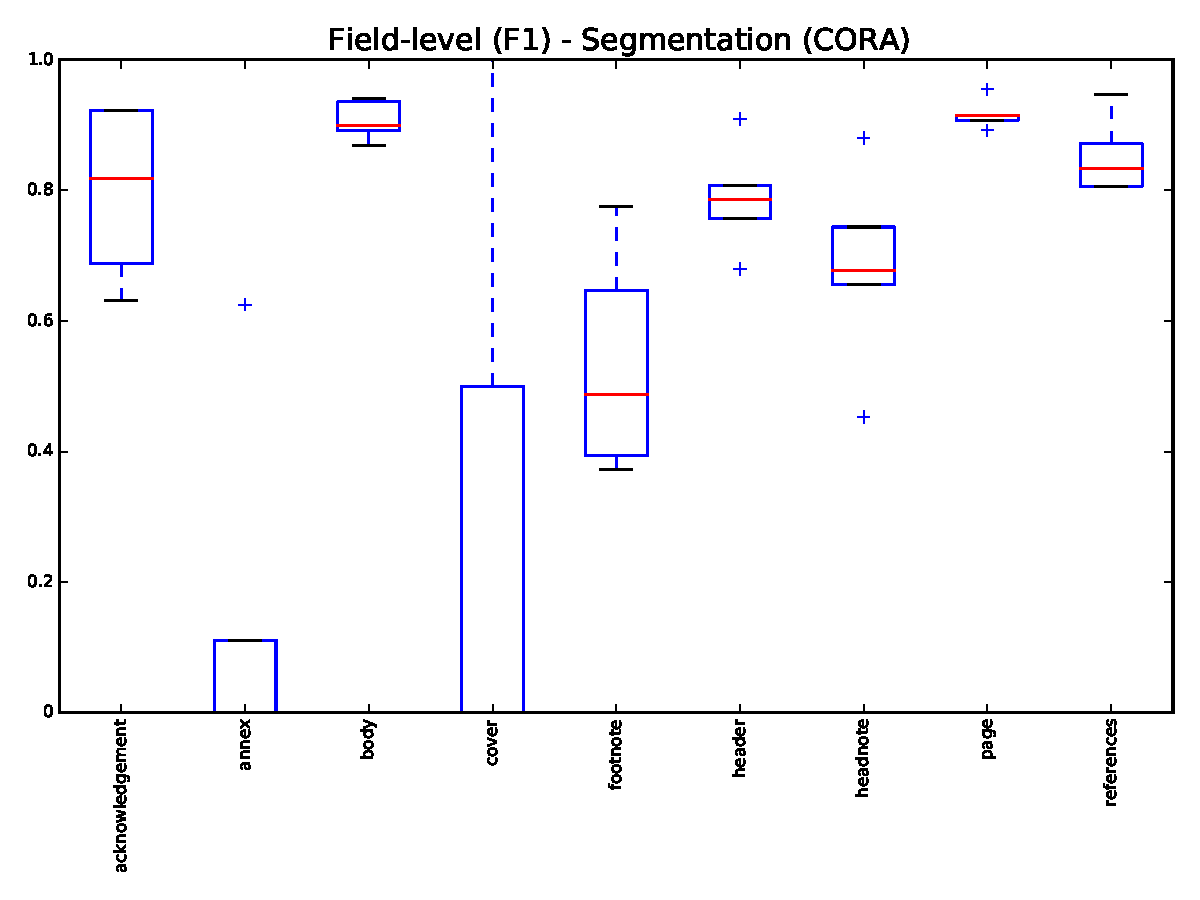
\includegraphics[width=0.75\textwidth]{../../figs/baseline/S_C/boxplot-field-level.pdf}}\\
%   \subfloat[][]{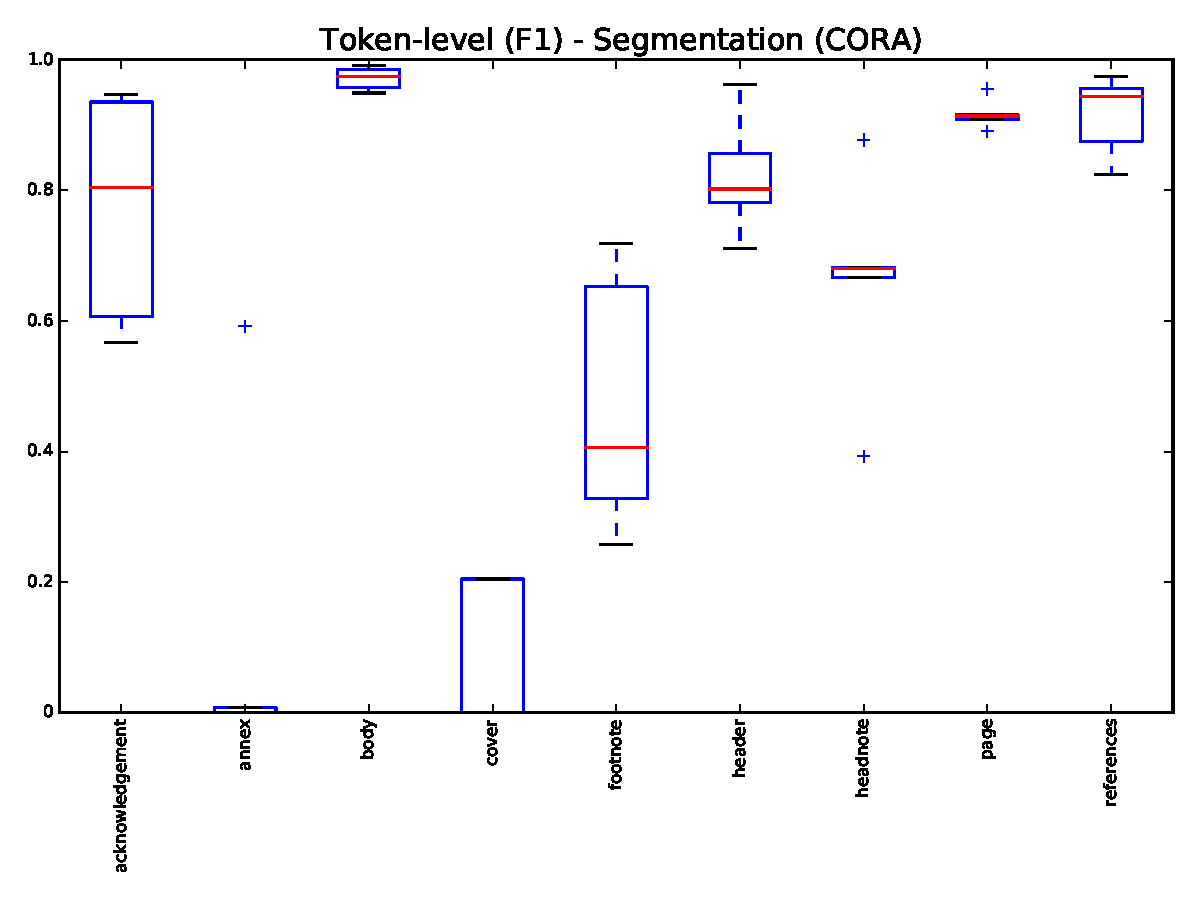
\includegraphics[width=0.75\textwidth]{../../figs/baseline/S_C/boxplot-token-level.pdf}}
% \end{figure}

% \begin{figure}[H]
%   \centering
%   \subfloat[][]{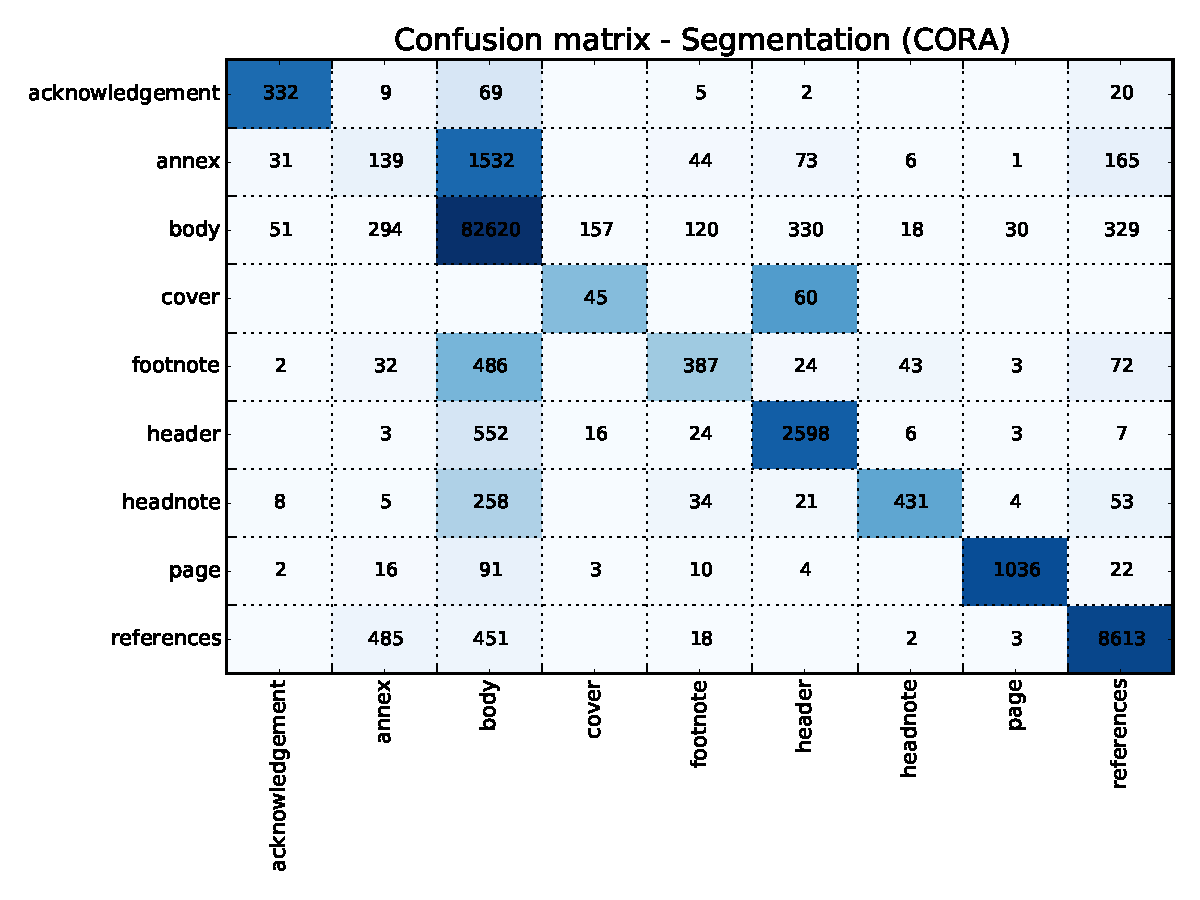
\includegraphics[width=0.75\textwidth]{../../figs/baseline/S_C/confusion_totals.pdf}}
% \end{figure}

% %%%%%%%%%%%%%%%%%%%%%%%%%%%%%%%%%%%%%%%%%%%%%%

% \subsubsection{Segmentation model - Cora dataset appending HEP dataset}

% %%%%%%%%%%%%%%%%%%%%%%%%%%%%%%%%%%%%%%%%%%%%%%

% \begin{figure}[H]
%   \centering
%   \subfloat[][]{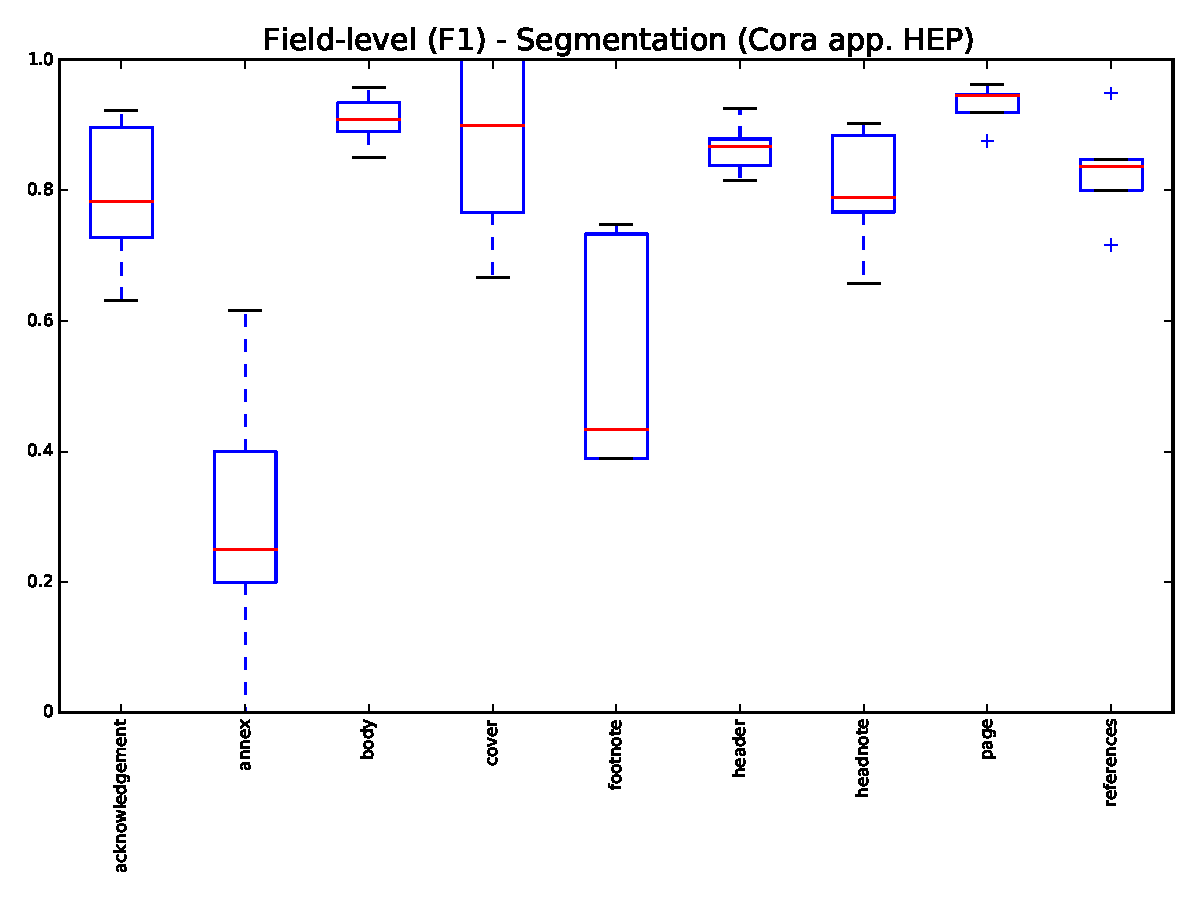
\includegraphics[width=0.75\textwidth]{../../figs/baseline/S_CappH/boxplot-field-level.pdf}}\\
%   \subfloat[][]{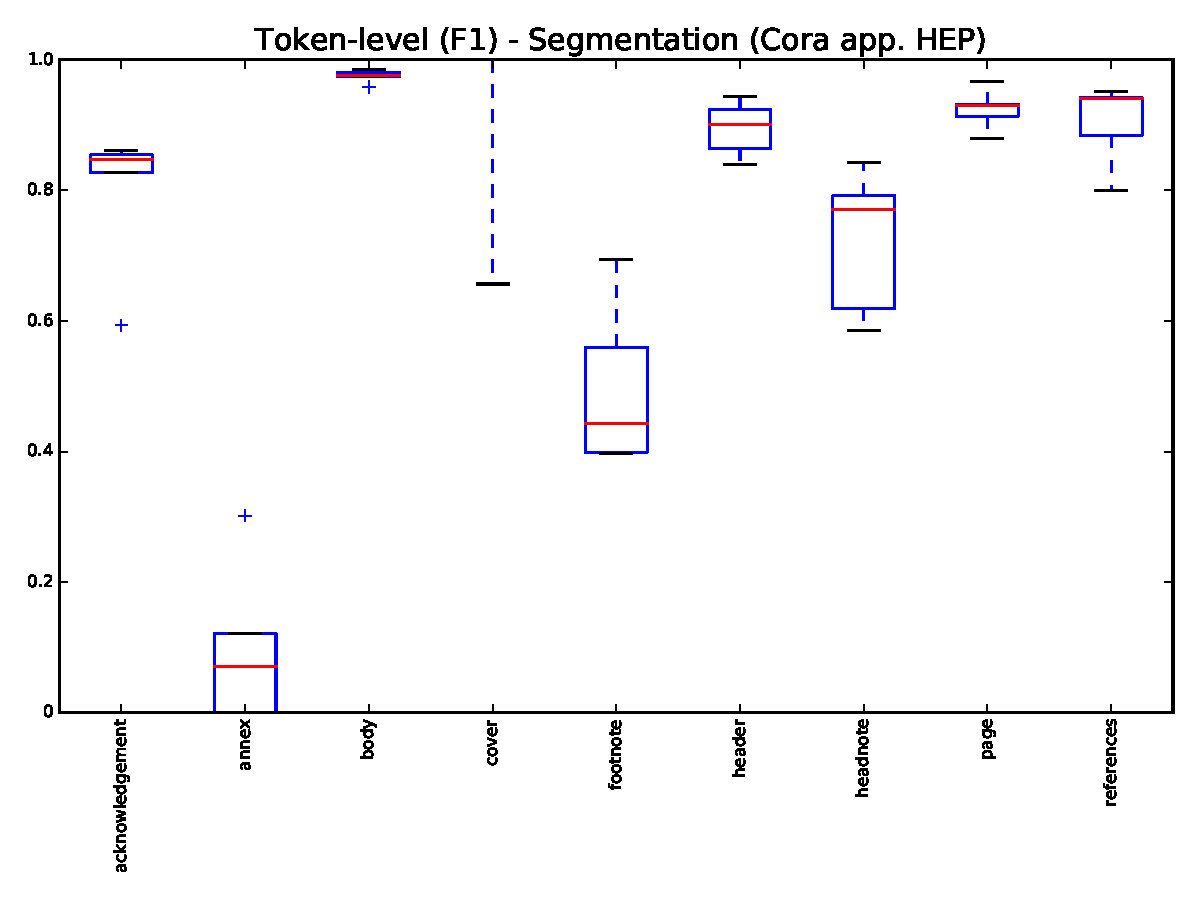
\includegraphics[width=0.75\textwidth]{../../figs/baseline/S_CappH/boxplot-token-level.pdf}}
% \end{figure}

% \begin{figure}[H]
%   \centering
%   \subfloat[][]{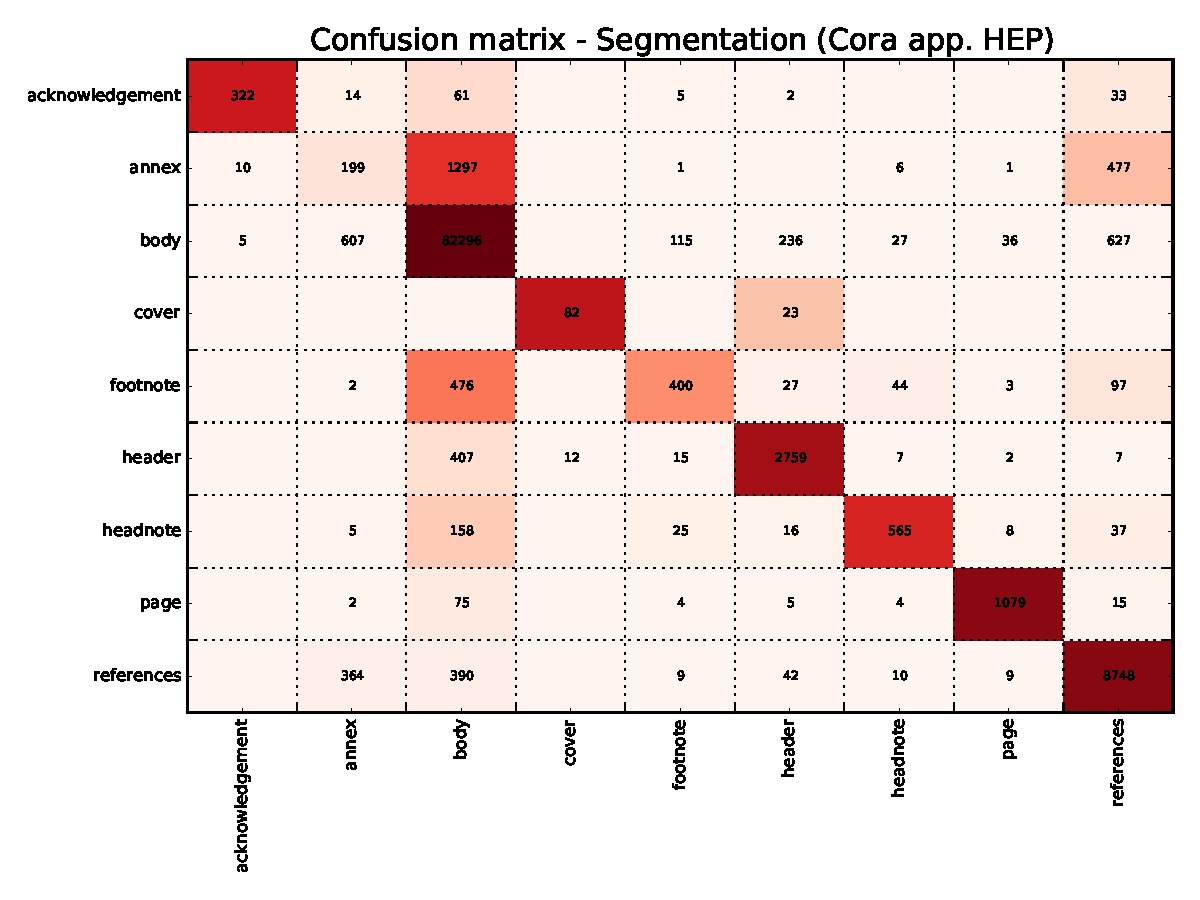
\includegraphics[width=0.75\textwidth]{../../figs/baseline/S_CappH/confusion_totals.pdf}}
% \end{figure}

% %%%%%%%%%%%%%%%%%%%%%%%%%%%%%%%%%%%%%%%%%%%%%%

% \subsubsection{Segmentation model - Cora and HEP combined datasets}

% %%%%%%%%%%%%%%%%%%%%%%%%%%%%%%%%%%%%%%%%%%%%%%

% \begin{figure}[H]
%   \centering
%   \subfloat[][]{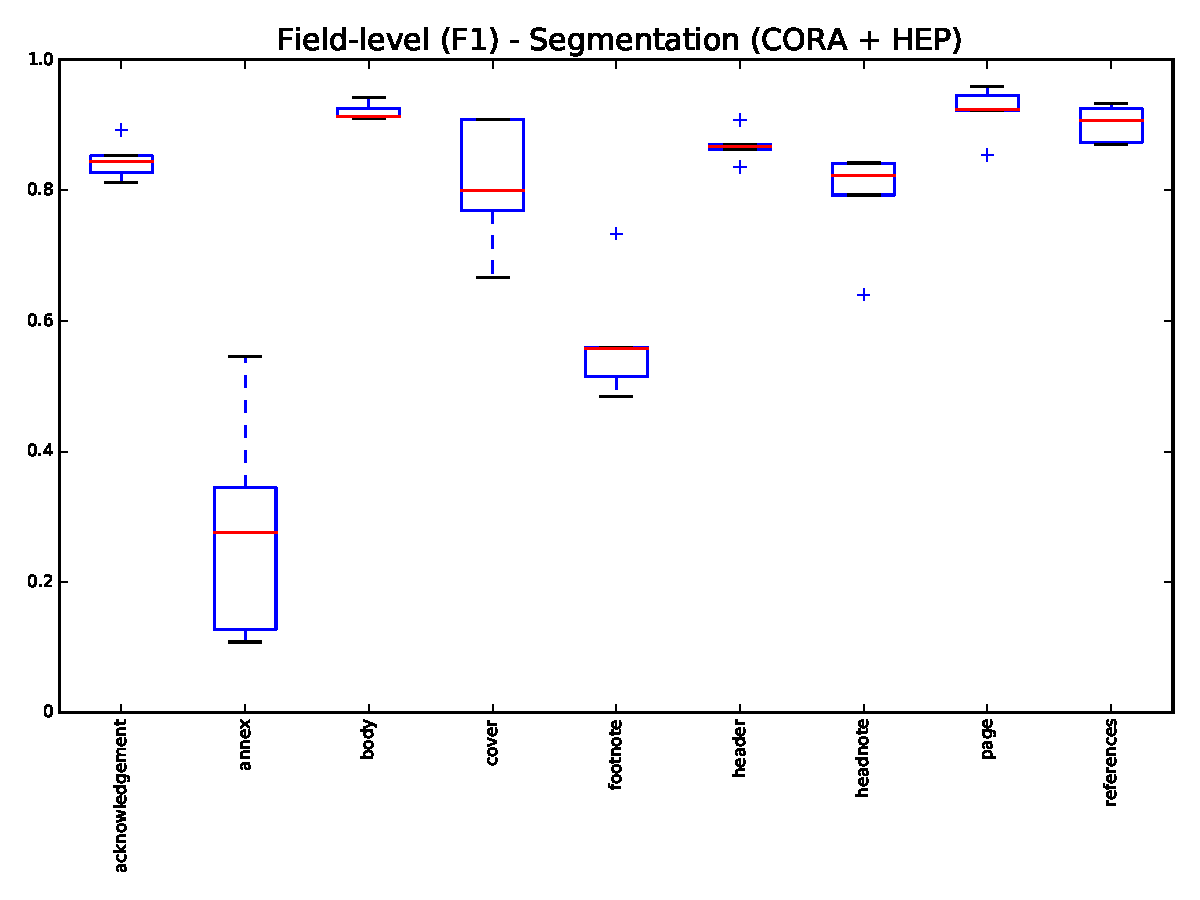
\includegraphics[width=0.75\textwidth]{../../figs/baseline/S_CH/boxplot-field-level.pdf}}\\
%   \subfloat[][]{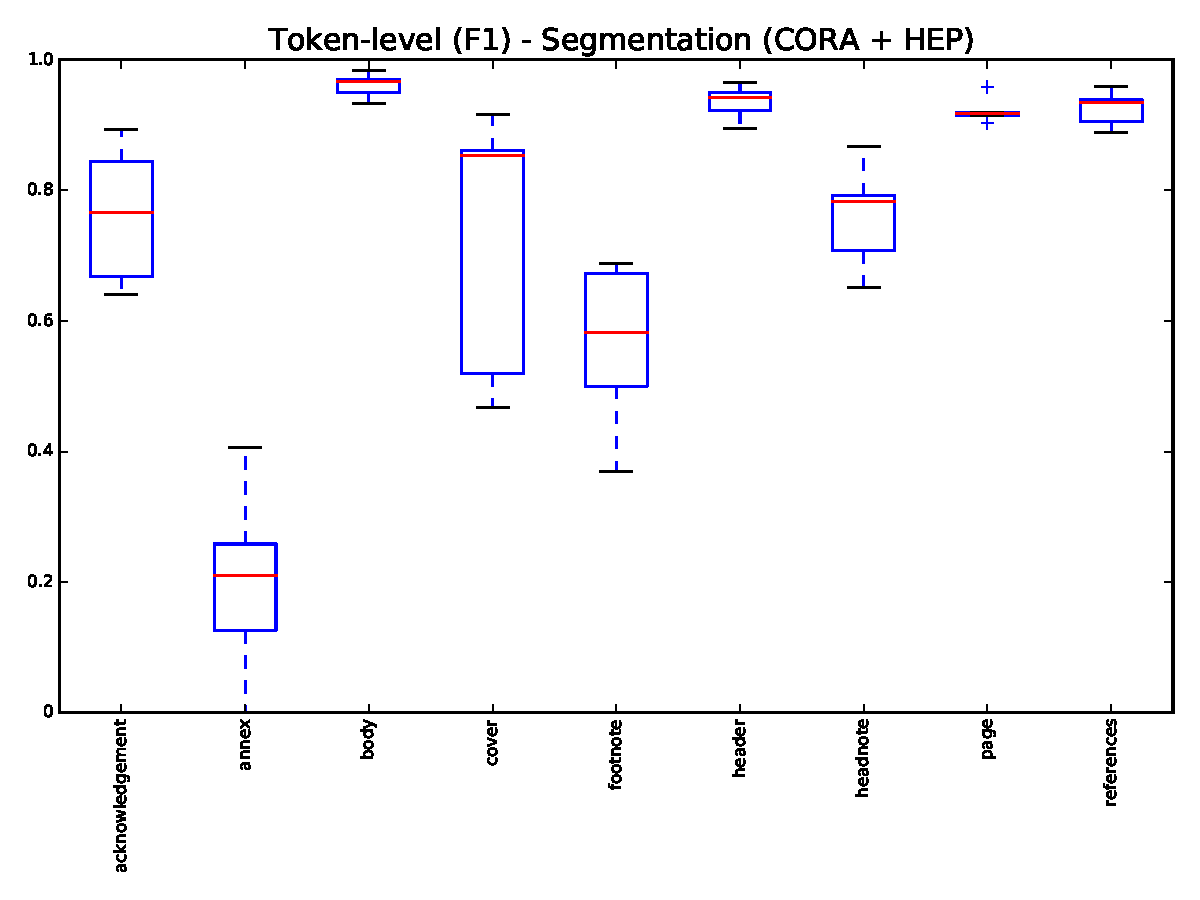
\includegraphics[width=0.75\textwidth]{../../figs/baseline/S_CH/boxplot-token-level.pdf}}
% \end{figure}

% \begin{figure}[H]
%   \centering
%   \subfloat[][]{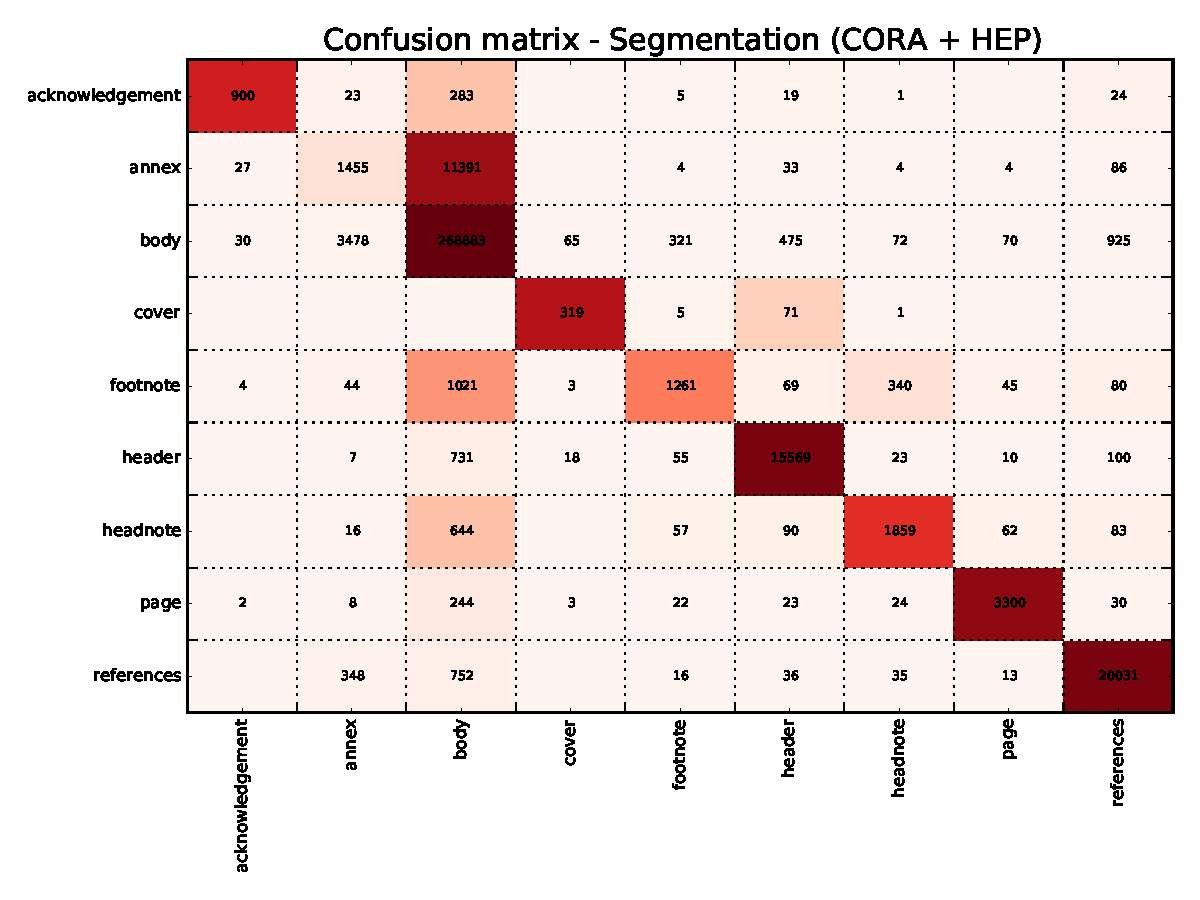
\includegraphics[width=0.75\textwidth]{../../figs/baseline/S_CH/confusion_totals.pdf}}
% \end{figure}

% %%%%%%%%%%%%%%%%%%%%%%%%%%%%%%%%%%%%%%%%%%%%%%

% \subsubsection{Segmentation model - HEP dataset}

% %%%%%%%%%%%%%%%%%%%%%%%%%%%%%%%%%%%%%%%%%%%%%%

% \begin{figure}[H]
%   \centering
%   \subfloat[][]{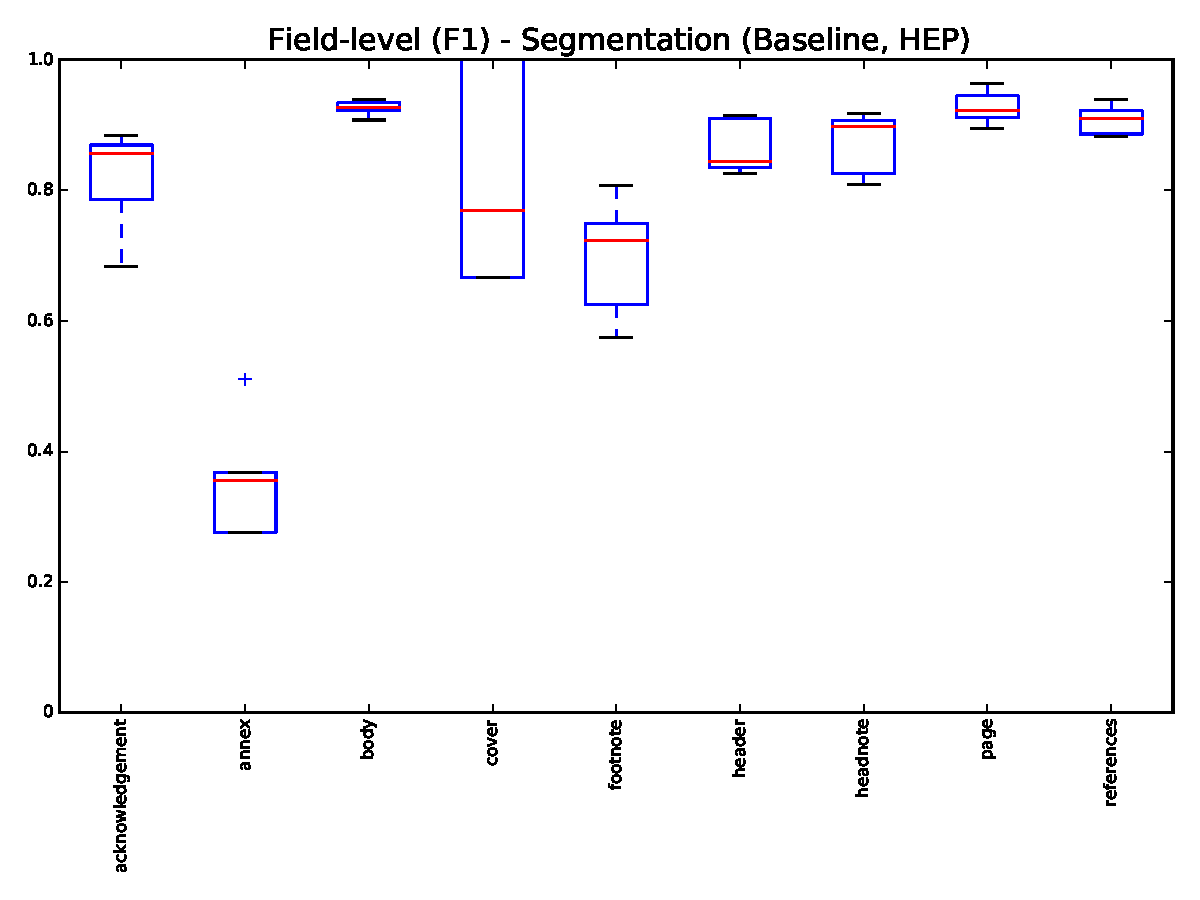
\includegraphics[width=0.75\textwidth]{../../figs/baseline/S_H/boxplot-field-level.pdf}}\\
%   \subfloat[][]{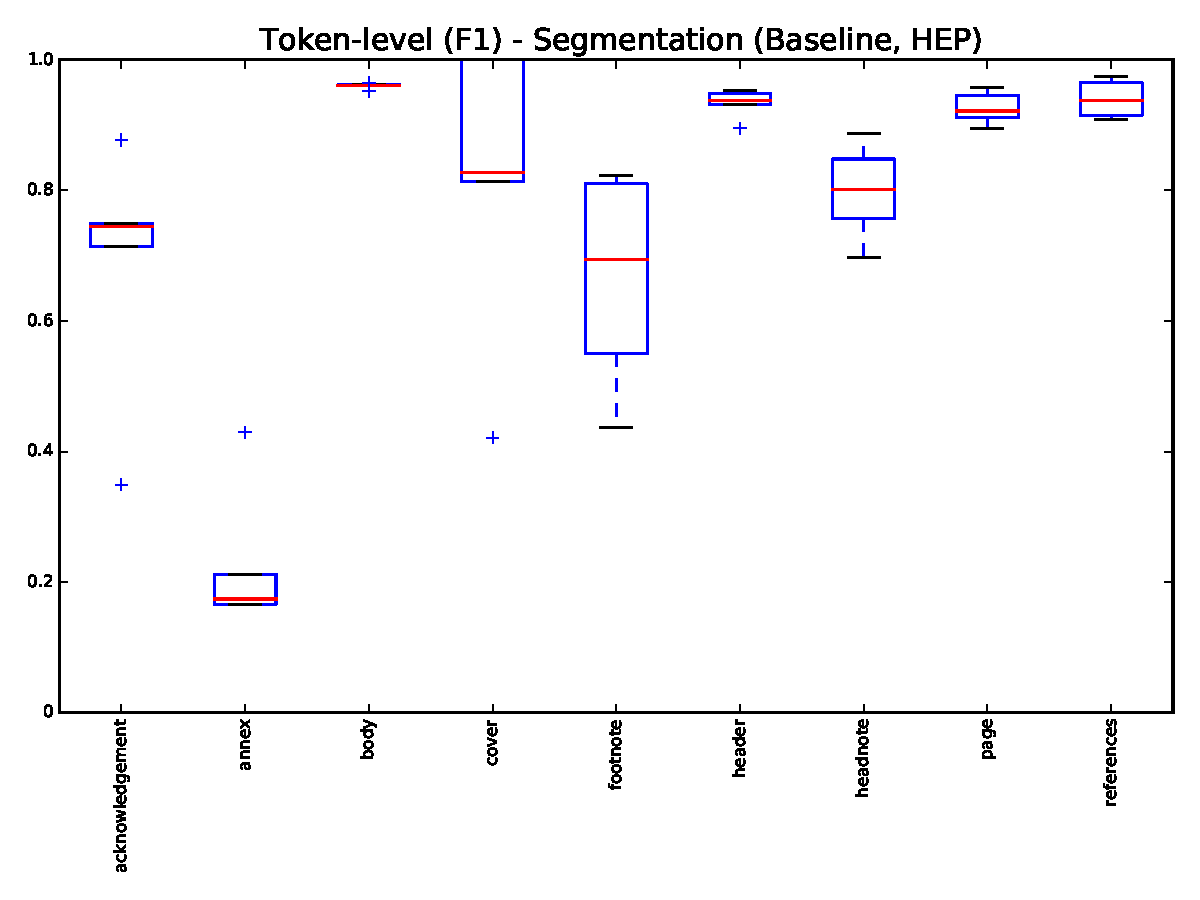
\includegraphics[width=0.75\textwidth]{../../figs/baseline/S_H/boxplot-token-level.pdf}}
% \end{figure}

% \begin{figure}[H]
%   \centering
%   \subfloat[][]{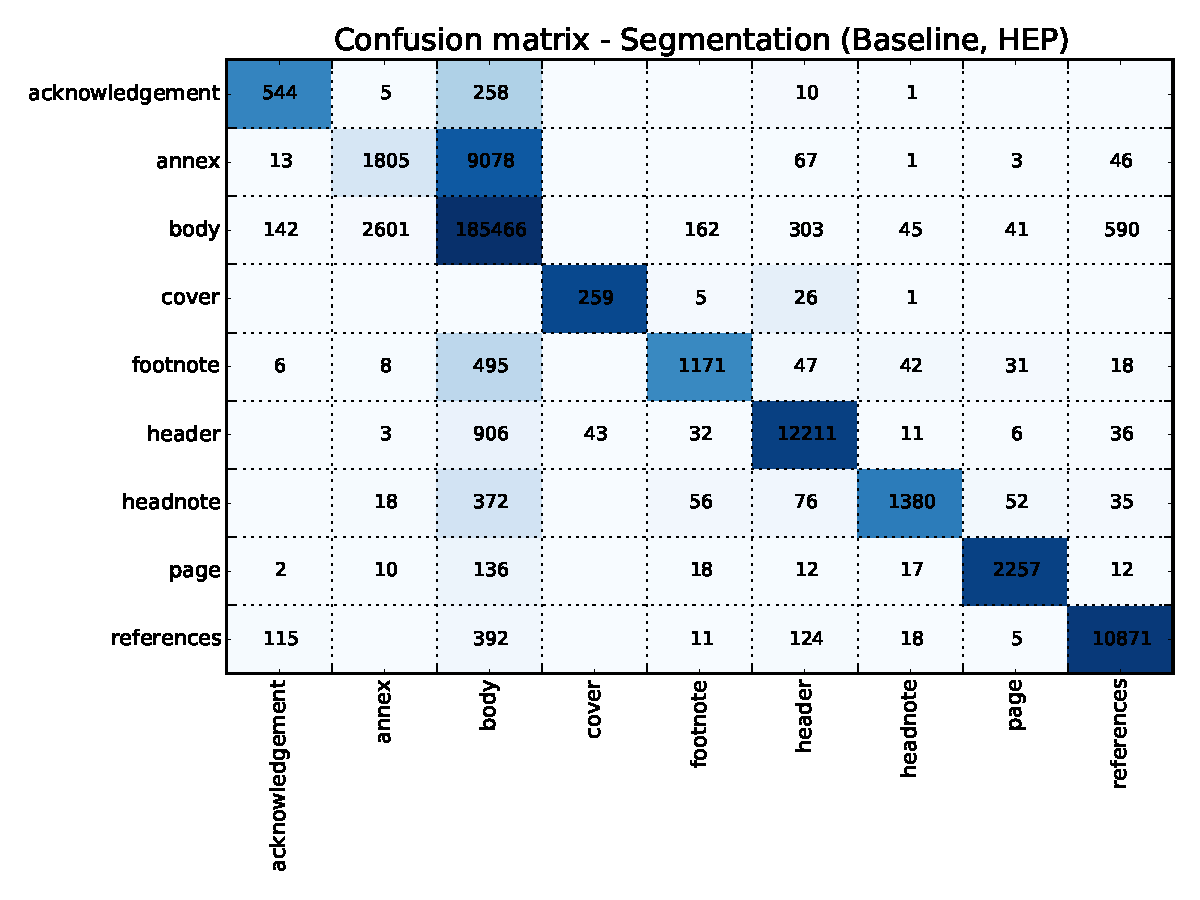
\includegraphics[width=0.75\textwidth]{../../figs/baseline/S_H/confusion_totals.pdf}}
% \end{figure}

% %%%%%%%%%%%%%%%%%%%%%%%%%%%%%%%%%%%%%%%%%%%%%%

% \subsubsection{Segmentation model - HEP dataset appending CORA dataset}

% %%%%%%%%%%%%%%%%%%%%%%%%%%%%%%%%%%%%%%%%%%%%%%

% \begin{figure}[H]
%   \centering
%   \subfloat[][]{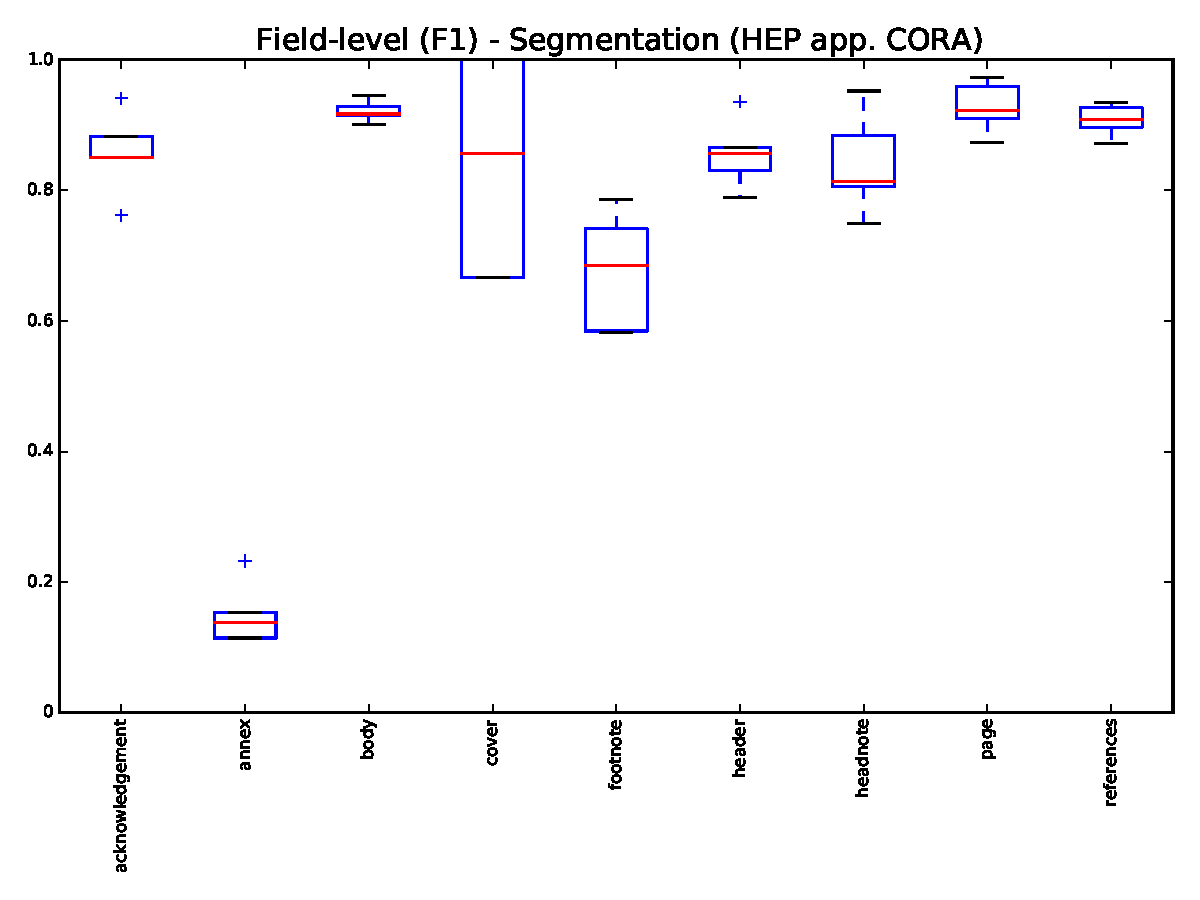
\includegraphics[width=0.75\textwidth]{../../figs/baseline/S_HappC/boxplot-field-level.pdf}}\\
%   \subfloat[][]{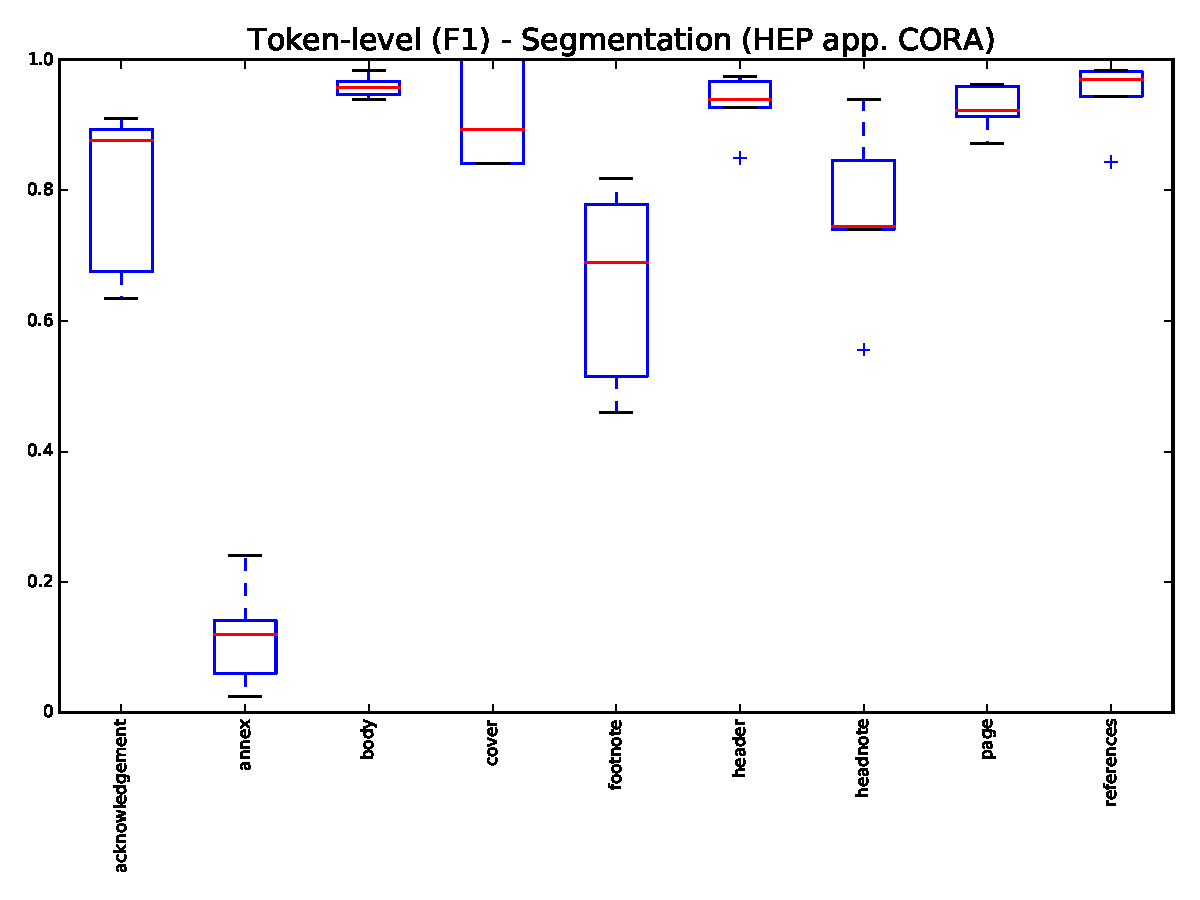
\includegraphics[width=0.75\textwidth]{../../figs/baseline/S_HappC/boxplot-token-level.pdf}}
% \end{figure}

% \begin{figure}[H]
%   \centering
%   \subfloat[][]{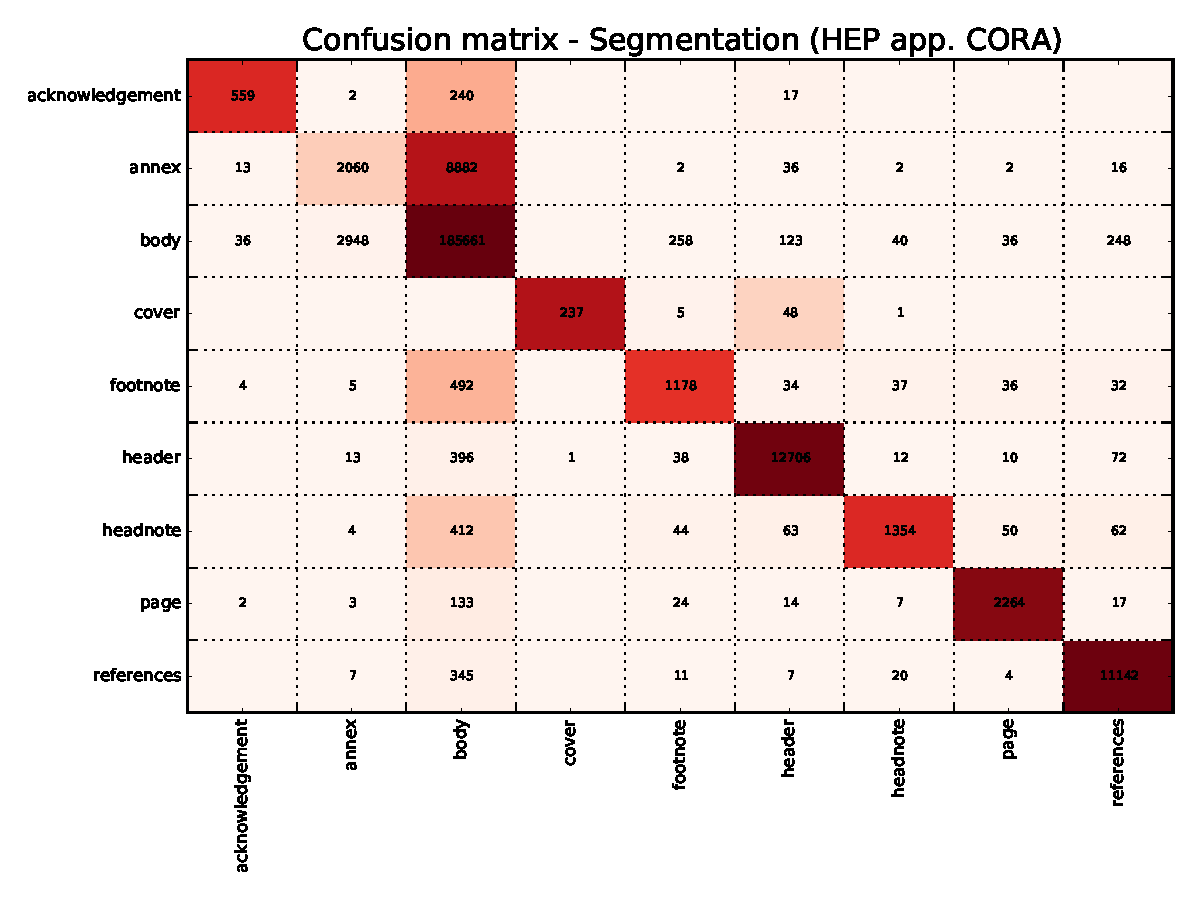
\includegraphics[width=0.75\textwidth]{../../figs/baseline/S_HappC/confusion_totals.pdf}}
% \end{figure}

% %%%%%%%%%%%%%%%%%%%%%%%%%%%%%%%%%%%%%%%%%%%%%%

% \subsection{Regularisation}
% \subsubsection{Header model - $L2 = 0$}

% %%%%%%%%%%%%%%%%%%%%%%%%%%%%%%%%%%%%%%%%%%%%%%

% \begin{figure}[H]
%   \centering
%   \subfloat[][]{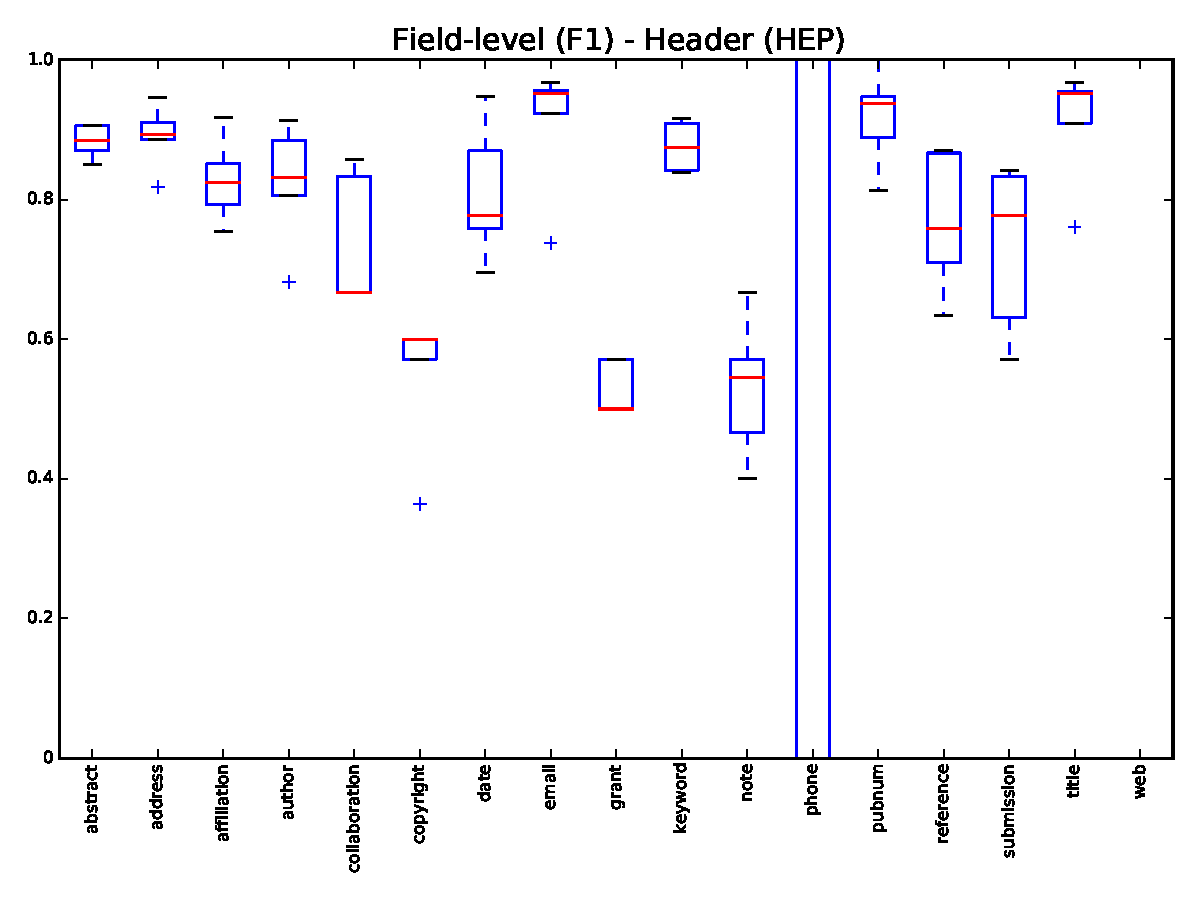
\includegraphics[width=0.75\textwidth]{../../figs/regularisation/H_H_L20/boxplot-field-level.pdf}}\\
%   \subfloat[][]{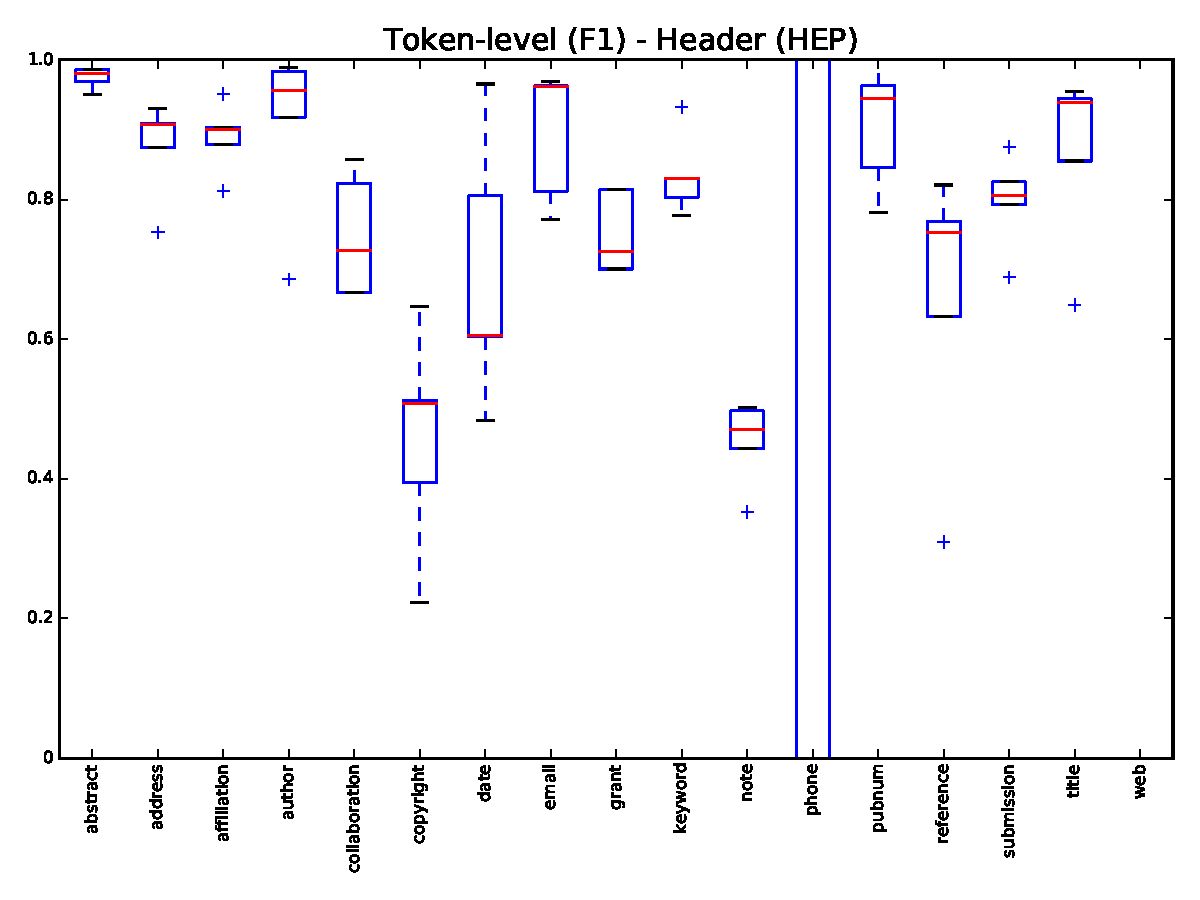
\includegraphics[width=0.75\textwidth]{../../figs/regularisation/H_H_L20/boxplot-token-level.pdf}}
% \end{figure}

% \begin{figure}[H]
%   \centering
%   \subfloat[][]{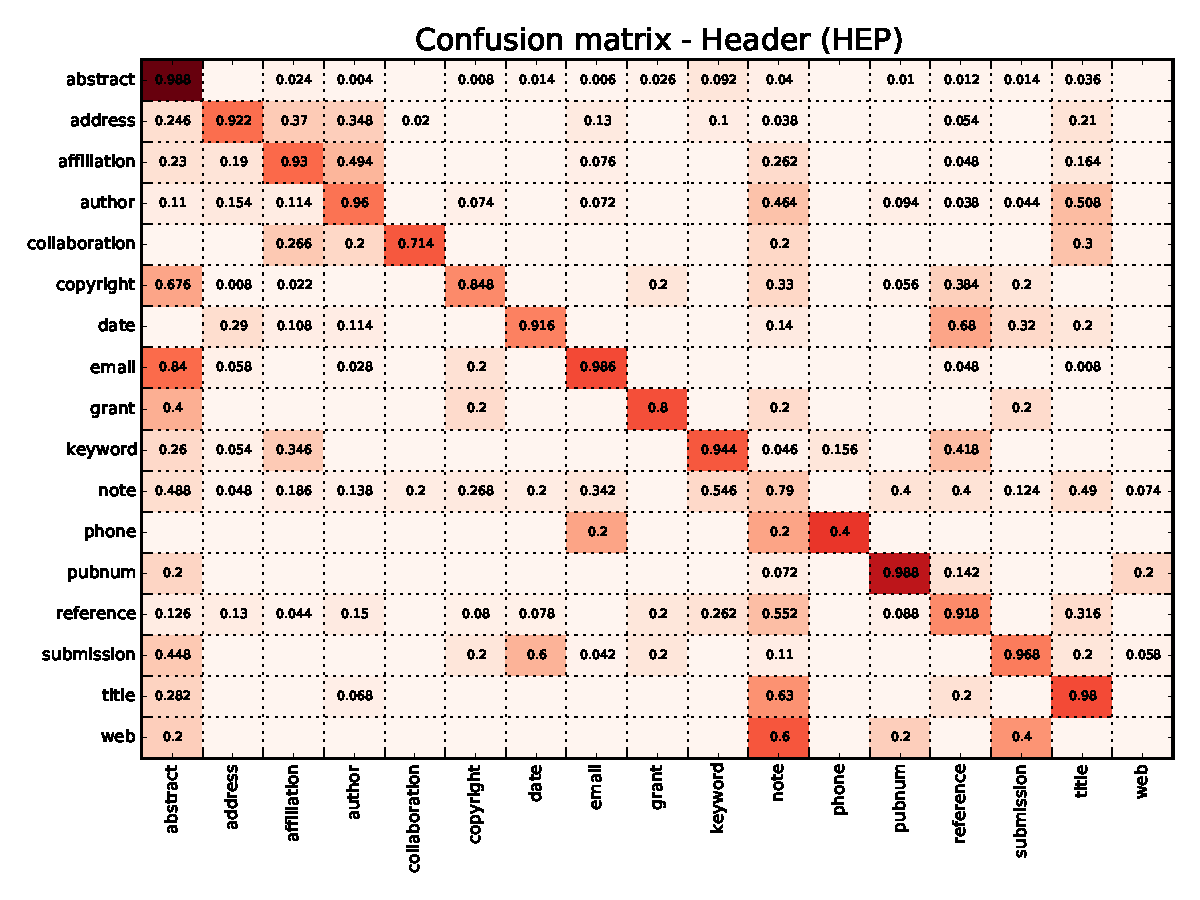
\includegraphics[width=0.75\textwidth]{../../figs/regularisation/H_H_L20/confusion_averages.pdf}}\\
%   \subfloat[][]{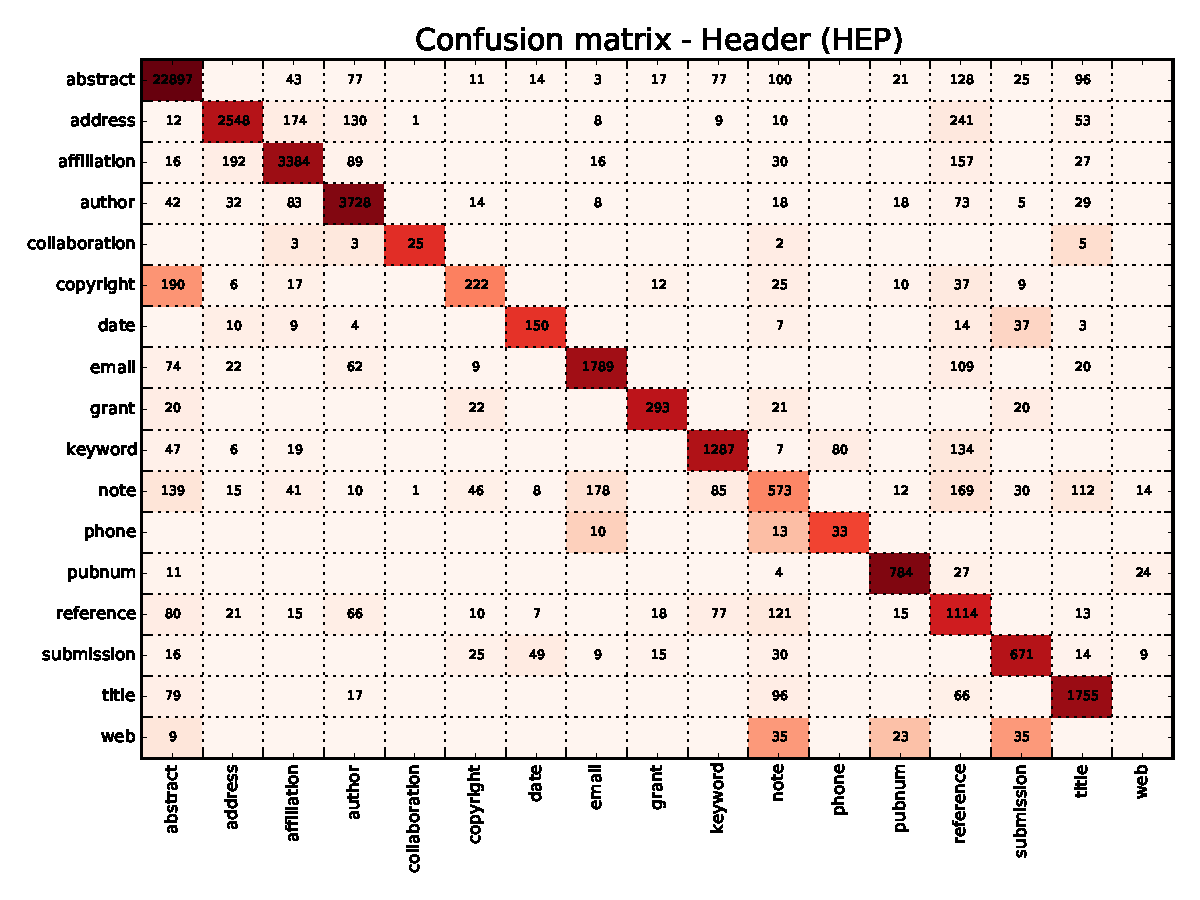
\includegraphics[width=0.75\textwidth]{../../figs/regularisation/H_H_L20/confusion_totals.pdf}}
% \end{figure}

% %%%%%%%%%%%%%%%%%%%%%%%%%%%%%%%%%%%%%%%%%%%%%%

% \subsubsection{Header model - $L2 = 1e^{-6}$}

% %%%%%%%%%%%%%%%%%%%%%%%%%%%%%%%%%%%%%%%%%%%%%%

% \begin{figure}[H]
%   \centering
%   \subfloat[][]{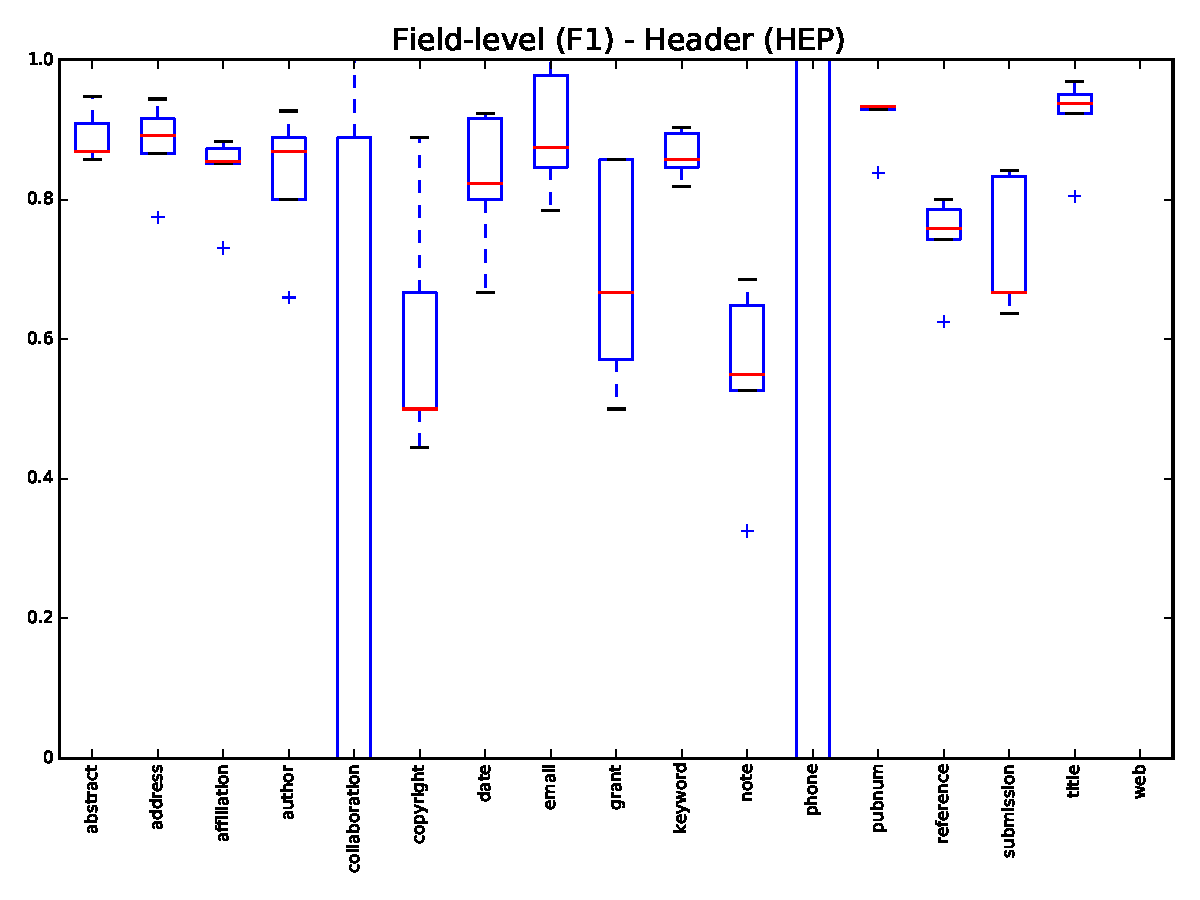
\includegraphics[width=0.75\textwidth]{../../figs/regularisation/H_H_L2e-6/boxplot-field-level.pdf}}\\
%   \subfloat[][]{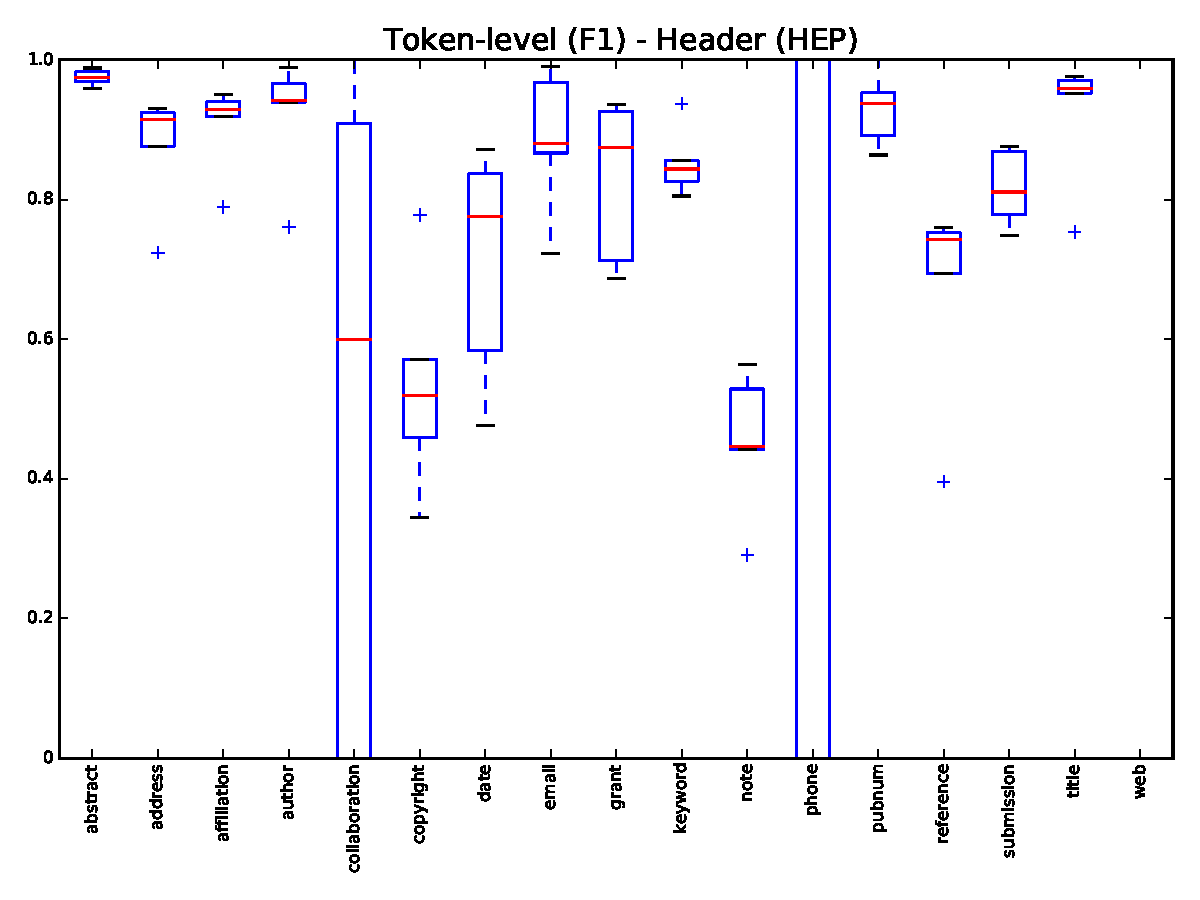
\includegraphics[width=0.75\textwidth]{../../figs/regularisation/H_H_L2e-6/boxplot-token-level.pdf}}
% \end{figure}

% \begin{figure}[H]
%   \centering
%   \subfloat[][]{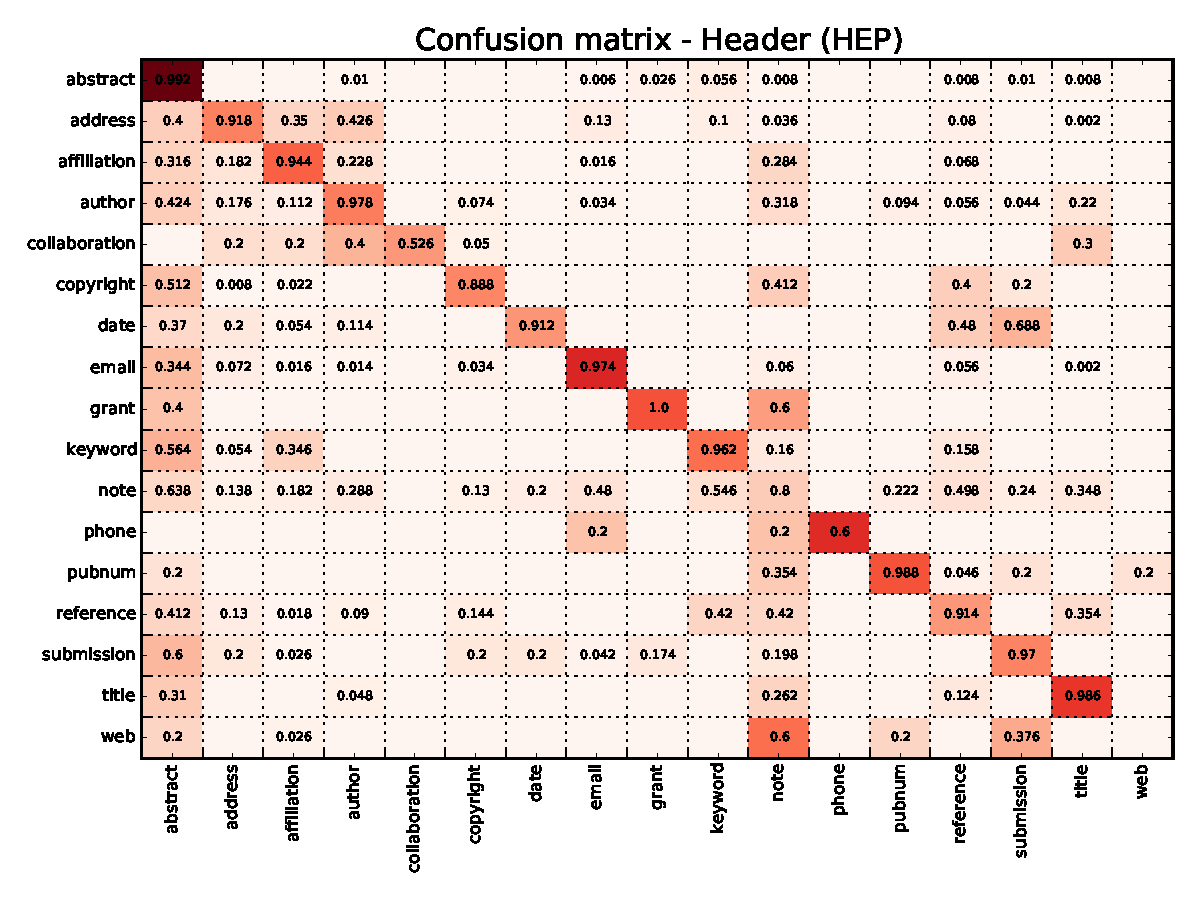
\includegraphics[width=0.75\textwidth]{../../figs/regularisation/H_H_L2e-6/confusion_averages.pdf}}\\
%   \subfloat[][]{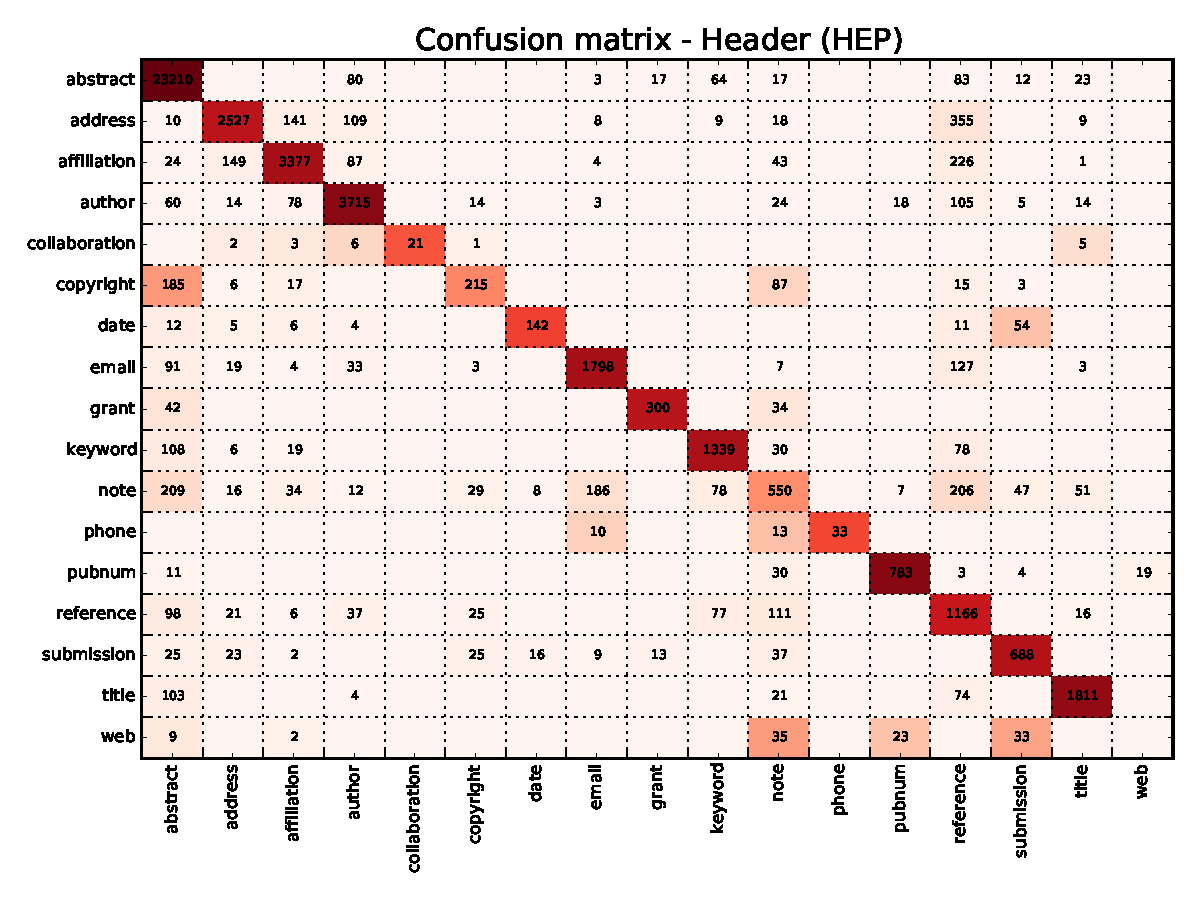
\includegraphics[width=0.75\textwidth]{../../figs/regularisation/H_H_L2e-6/confusion_totals.pdf}}
% \end{figure}

% %%%%%%%%%%%%%%%%%%%%%%%%%%%%%%%%%%%%%%%%%%%%%%

% \subsubsection{Header model - $L2 = 1e^{-5}$}

% %%%%%%%%%%%%%%%%%%%%%%%%%%%%%%%%%%%%%%%%%%%%%%

% \begin{figure}[H]
%   \centering
%   \subfloat[][]{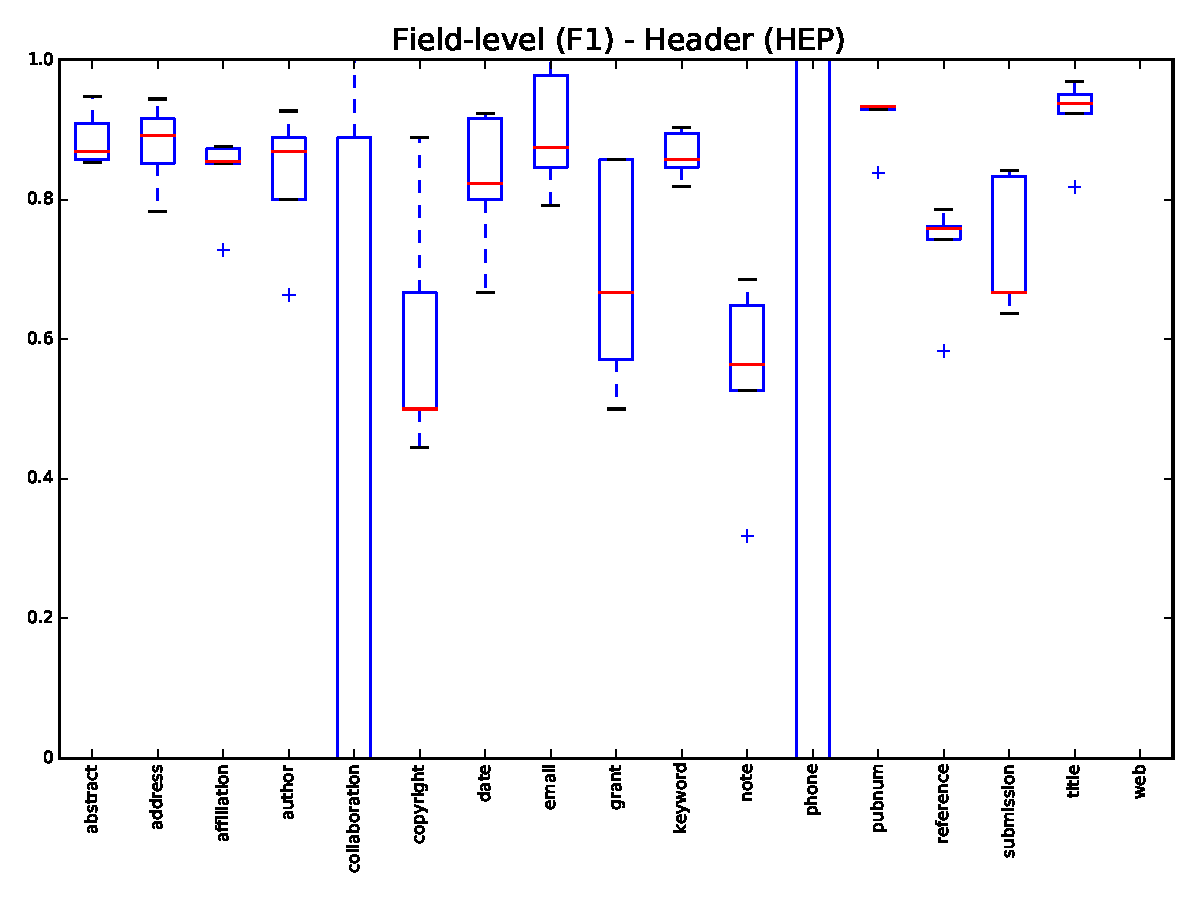
\includegraphics[width=0.75\textwidth]{../../figs/regularisation/H_H_L2e-5/boxplot-field-level.pdf}}\\
%   \subfloat[][]{\includegraphics[width=0.75\textwidth]{../../figs/regularisation/H_H_L2e-5/boxplot-token-level.pdf}}
% \end{figure}

% \begin{figure}[H]
%   \centering
%   \subfloat[][]{\includegraphics[width=0.75\textwidth]{../../figs/regularisation/H_H_L2e-5/confusion_averages.pdf}}\\
%   \subfloat[][]{\includegraphics[width=0.75\textwidth]{../../figs/regularisation/H_H_L2e-5/confusion_totals.pdf}}
% \end{figure}

% %%%%%%%%%%%%%%%%%%%%%%%%%%%%%%%%%%%%%%%%%%%%%%

% \subsubsection{Header model - $L2 = 1e^{-4}$}

% %%%%%%%%%%%%%%%%%%%%%%%%%%%%%%%%%%%%%%%%%%%%%%

% \begin{figure}[H]
%   \centering
%   \subfloat[][]{\includegraphics[width=0.75\textwidth]{../../figs/regularisation/H_H_L2e-4/boxplot-field-level.pdf}}\\
%   \subfloat[][]{\includegraphics[width=0.75\textwidth]{../../figs/regularisation/H_H_L2e-4/boxplot-token-level.pdf}}
% \end{figure}

% \begin{figure}[H]
%   \centering
%   \subfloat[][]{\includegraphics[width=0.75\textwidth]{../../figs/regularisation/H_H_L2e-4/confusion_averages.pdf}}\\
%   \subfloat[][]{\includegraphics[width=0.75\textwidth]{../../figs/regularisation/H_H_L2e-4/confusion_totals.pdf}}
% \end{figure}

% %%%%%%%%%%%%%%%%%%%%%%%%%%%%%%%%%%%%%%%%%%%%%%

% \subsubsection{Header model - $L2 = 1e^{-3}$}

% %%%%%%%%%%%%%%%%%%%%%%%%%%%%%%%%%%%%%%%%%%%%%%

% \begin{figure}[H]
%   \centering
%   \subfloat[][]{\includegraphics[width=0.75\textwidth]{../../figs/regularisation/H_H_L2e-3/boxplot-field-level.pdf}}\\
%   \subfloat[][]{\includegraphics[width=0.75\textwidth]{../../figs/regularisation/H_H_L2e-3/boxplot-token-level.pdf}}
% \end{figure}

% \begin{figure}[H]
%   \centering
%   \subfloat[][]{\includegraphics[width=0.75\textwidth]{../../figs/regularisation/H_H_L2e-3/confusion_averages.pdf}}\\
%   \subfloat[][]{\includegraphics[width=0.75\textwidth]{../../figs/regularisation/H_H_L2e-3/confusion_totals.pdf}}
% \end{figure}

% %%%%%%%%%%%%%%%%%%%%%%%%%%%%%%%%%%%%%%%%%%%%%%

% \subsection{Dictionaries}
% \subsubsection{Header model - HEP dataset}

% %%%%%%%%%%%%%%%%%%%%%%%%%%%%%%%%%%%%%%%%%%%%%%

% \begin{figure}[H]
%   \centering
%   \subfloat[][]{\includegraphics[width=0.75\textwidth]{../../figs/dicts/H_H_dicts/boxplot-field-level.pdf}}\\
%   \subfloat[][]{\includegraphics[width=0.75\textwidth]{../../figs/dicts/H_H_dicts/boxplot-token-level.pdf}}
% \end{figure}

% \begin{figure}[H]
%   \centering
%   \subfloat[][]{\includegraphics[width=0.75\textwidth]{../../figs/dicts/H_H_dicts/confusion_averages.pdf}}\\
%   \subfloat[][]{\includegraphics[width=0.75\textwidth]{../../figs/dicts/H_H_dicts/confusion_totals.pdf}}
% \end{figure}

% %%%%%%%%%%%%%%%%%%%%%%%%%%%%%%%%%%%%%%%%%%%%%%

% \subsubsection{Header model - HEP dataset appending CORA dataset}

% %%%%%%%%%%%%%%%%%%%%%%%%%%%%%%%%%%%%%%%%%%%%%%

% \begin{figure}[H]
%   \centering
%   \subfloat[][]{\includegraphics[width=0.75\textwidth]{../../figs/dicts/H_HappC_dicts/boxplot-field-level.pdf}}\\
%   \subfloat[][]{\includegraphics[width=0.75\textwidth]{../../figs/dicts/H_HappC_dicts/boxplot-token-level.pdf}}
% \end{figure}

% \begin{figure}[H]
%   \centering
%   \subfloat[][]{\includegraphics[width=0.75\textwidth]{../../figs/dicts/H_HappC_dicts/confusion_averages.pdf}}\\
%   \subfloat[][]{\includegraphics[width=0.75\textwidth]{../../figs/dicts/H_HappC_dicts/confusion_totals.pdf}}
% \end{figure}

% %%%%%%%%%%%%%%%%%%%%%%%%%%%%%%%%%%%%%%%%%%%%%%

% \subsubsection{Segmentation model - HEP dataset}

% %%%%%%%%%%%%%%%%%%%%%%%%%%%%%%%%%%%%%%%%%%%%%%

% \begin{figure}[H]
%   \centering
%   \subfloat[][]{\includegraphics[width=0.75\textwidth]{../../figs/dicts/S_H_dicts/boxplot-field-level.pdf}}\\
%   \subfloat[][]{\includegraphics[width=0.75\textwidth]{../../figs/dicts/S_H_dicts/boxplot-token-level.pdf}}
% \end{figure}

% \begin{figure}[H]
%   \centering
%   \subfloat[][]{\includegraphics[width=0.75\textwidth]{../../figs/dicts/S_H_dicts/confusion_averages.pdf}}\\
%   \subfloat[][]{\includegraphics[width=0.75\textwidth]{../../figs/dicts/S_H_dicts/confusion_totals.pdf}}
% \end{figure}

% %%%%%%%%%%%%%%%%%%%%%%%%%%%%%%%%%%%%%%%%%%%%%%

% \subsubsection{Segmentation model - HEP dataset appending CORA dataset}

% %%%%%%%%%%%%%%%%%%%%%%%%%%%%%%%%%%%%%%%%%%%%%%

% \begin{figure}[H]
%   \centering
%   \subfloat[][]{\includegraphics[width=0.75\textwidth]{../../figs/dicts/S_HappC_dicts/boxplot-field-level.pdf}}\\
%   \subfloat[][]{\includegraphics[width=0.75\textwidth]{../../figs/dicts/S_HappC_dicts/boxplot-token-level.pdf}}
% \end{figure}

% \begin{figure}[H]
%   \centering
%   \subfloat[][]{\includegraphics[width=0.75\textwidth]{../../figs/dicts/S_HappC_dicts/confusion_averages.pdf}}\\
%   \subfloat[][]{\includegraphics[width=0.75\textwidth]{../../figs/dicts/S_HappC_dicts/confusion_totals.pdf}}
% \end{figure}

% %%%%%%%%%%%%%%%%%%%%%%%%%%%%%%%%%%%%%%%%%%%%%%

% \subsubsection{Header Model - HEP dataset - $2^{nd}$ Degree Features}
% \subsubsection{Header Model - HEP dataset Appending CORA - $2^{nd}$ Degree Features}
% \subsubsection{Header Model - HEP dataset - $3^{rd}$ Degree Features}
% \subsubsection{Header Model - HEP dataset Appending CORA - $3^{rd}$ Degree Features}

% \subsection{Dictionaries + stop words}
% \subsubsection{Header model - HEP dataset}

% %%%%%%%%%%%%%%%%%%%%%%%%%%%%%%%%%%%%%%%%%%%%%%

% \begin{figure}[H]
%   \centering
%   \subfloat[][]{\includegraphics[width=0.75\textwidth]{../../figs/dicts_stops/H_H_dicts_stops/boxplot-field-level.pdf}}\\
%   \subfloat[][]{\includegraphics[width=0.75\textwidth]{../../figs/dicts_stops/H_H_dicts_stops/boxplot-token-level.pdf}}
% \end{figure}

% \begin{figure}[H]
%   \centering
%   \subfloat[][]{\includegraphics[width=0.75\textwidth]{../../figs/dicts_stops/H_H_dicts_stops/confusion_averages.pdf}}\\
%   \subfloat[][]{\includegraphics[width=0.75\textwidth]{../../figs/dicts_stops/H_H_dicts_stops/confusion_totals.pdf}}
% \end{figure}

% %%%%%%%%%%%%%%%%%%%%%%%%%%%%%%%%%%%%%%%%%%%%%%

% \subsubsection{Header model - HEP dataset appending CORA dataset}

% %%%%%%%%%%%%%%%%%%%%%%%%%%%%%%%%%%%%%%%%%%%%%%

% \begin{figure}[H]
%   \centering
%   \subfloat[][]{\includegraphics[width=0.75\textwidth]{../../figs/dicts_stops/H_HappC_dicts_stops/boxplot-field-level.pdf}}\\
%   \subfloat[][]{\includegraphics[width=0.75\textwidth]{../../figs/dicts_stops/H_HappC_dicts_stops/boxplot-token-level.pdf}}
% \end{figure}

% \begin{figure}[H]
%   \centering
%   \subfloat[][]{\includegraphics[width=0.75\textwidth]{../../figs/dicts_stops/H_HappC_dicts_stops/confusion_averages.pdf}}\\
%   \subfloat[][]{\includegraphics[width=0.75\textwidth]{../../figs/dicts_stops/H_HappC_dicts_stops/confusion_totals.pdf}}
% \end{figure}

% %%%%%%%%%%%%%%%%%%%%%%%%%%%%%%%%%%%%%%%%%%%%%%

% \subsubsection{Segmentation model - HEP dataset}

% %%%%%%%%%%%%%%%%%%%%%%%%%%%%%%%%%%%%%%%%%%%%%%

% \begin{figure}[H]
%   \centering
%   \subfloat[][]{\includegraphics[width=0.75\textwidth]{../../figs/dicts_stops/S_H_dicts_stops/boxplot-field-level.pdf}}\\
%   \subfloat[][]{\includegraphics[width=0.75\textwidth]{../../figs/dicts_stops/S_H_dicts_stops/boxplot-token-level.pdf}}
% \end{figure}

% \begin{figure}[H]
%   \centering
%   \subfloat[][]{\includegraphics[width=0.75\textwidth]{../../figs/dicts_stops/S_H_dicts_stops/confusion_averages.pdf}}\\
%   \subfloat[][]{\includegraphics[width=0.75\textwidth]{../../figs/dicts_stops/S_H_dicts_stops/confusion_totals.pdf}}
% \end{figure}

% %%%%%%%%%%%%%%%%%%%%%%%%%%%%%%%%%%%%%%%%%%%%%%

% \subsubsection{Segmentation model - HEP dataset appending CORA dataset}

% %%%%%%%%%%%%%%%%%%%%%%%%%%%%%%%%%%%%%%%%%%%%%%

% \begin{figure}[H]
%   \centering
%   \subfloat[][]{\includegraphics[width=0.75\textwidth]{../../figs/dicts_stops/S_HappC_dicts_stops/boxplot-field-level.pdf}}\\
%   \subfloat[][]{\includegraphics[width=0.75\textwidth]{../../figs/dicts_stops/S_HappC_dicts_stops/boxplot-token-level.pdf}}
% \end{figure}

% \begin{figure}[H]
%   \centering
%   \subfloat[][]{\includegraphics[width=0.75\textwidth]{../../figs/dicts_stops/S_HappC_dicts_stops/confusion_averages.pdf}}\\
%   \subfloat[][]{\includegraphics[width=0.75\textwidth]{../../figs/dicts_stops/S_HappC_dicts_stops/confusion_totals.pdf}}
% \end{figure}

% %%%%%%%%%%%%%%%%%%%%%%%%%%%%%%%%%%%%%%%%%%%%%%

% \subsubsection{Header Model - HEP dataset - $2^{nd}$ Degree Features}
% \subsubsection{Header Model - HEP dataset Appending CORA - $2^{nd}$ Degree Features}
% \subsubsection{Header Model - HEP dataset - $3^{rd}$ Degree Features}
% \subsubsection{Header Model - HEP dataset Appending CORA - $3^{rd}$ Degree Features}

% \subsection{Token Selection}
% \subsubsection{Segmentation Model - HEP dataset - 5 Tokens}
% \subsubsection{Segmentation Model - HEP dataset - 10 Tokens}
% \subsubsection{Segmentation Model - HEP dataset - 15 Tokens}
% \subsubsection{Segmentation Model - HEP dataset - 20 Tokens}

% \subsection{Levenshtein}
% \subsubsection{Segmentation Model - HEP dataset - Binary Threshold (0.05)}
% \subsubsection{Segmentation Model - HEP dataset - Binary Threshold (0.1)}
% \subsubsection{Segmentation Model - HEP dataset - Binary Threshold (0.2)}
% \subsubsection{Segmentation Model - HEP dataset - Binary Threshold (0.4)}
% \subsubsection{Segmentation Model - HEP dataset - Binary Threshold (0.8)}
% \subsubsection{Segmentation Model - HEP dataset - Ternary Threshold}
% \subsubsection{Segmentation Model - HEP dataset - Quaternary Threshold}

% \subsection{Line Shape}
% \subsubsection{Segmentation Model - HEP dataset - Binary Threshold}
% \subsubsection{Segmentation Model - HEP dataset - Ternary Threshold}

% \subsection{Template Matching}
% \subsubsection{Segmentation Model - HEP dataset}

% \section{Conclusion}
% \subsection{Summary}
% \subsubsection{Key Results}
% \subsection{Future Work}

% \section{References}
% % http://dblp.uni-trier.de/

% \section{Appendices}

\bibliographystyle{plain}
\bibliography{refs}

\end{document}